% ==============================================================================
%  SEP490_04 FA26 -- FREVIA Graduation Defense Presentation
%  Compiler: xelatex (run twice for page numbers)
% ==============================================================================
\documentclass[aspectratio=169,11pt]{beamer}

\usepackage{fontspec}
\usepackage{xcolor}
\usepackage{graphicx}
\usepackage{tikz}
\usepackage{booktabs}
\usepackage{array}
\usepackage{colortbl}
\usepackage{tabularx}
\usepackage{amsmath}
\usetikzlibrary{shapes,arrows.meta,positioning,calc}

% ── Fonts ──────────────────────────────────────────────────────────────────────
\setmainfont{Arial}
\setsansfont{Arial}
\setmonofont{Consolas}[Scale=0.85]

% ── FPT Dark-Navy Theme Palette ────────────────────────────────────────────────
\definecolor{fptnavy}{RGB}{8,26,64}
\definecolor{fptnavylight}{RGB}{16,42,96}
\definecolor{fptcard}{RGB}{14,36,84}
\definecolor{fptblue}{RGB}{0,82,180}
\definecolor{fptaccent}{RGB}{56,163,255}
\definecolor{fptteal}{RGB}{0,200,210}
\definecolor{fptgold}{RGB}{255,190,40}
\definecolor{successgreen}{RGB}{34,197,94}
\definecolor{lightgray}{RGB}{200,214,232}
\definecolor{mutedgray}{RGB}{145,165,195}

% ── Beamer Layout & Styling ────────────────────────────────────────────────────
\usetheme{default}
\setbeamertemplate{navigation symbols}{}
\setbeamercolor{background canvas}{bg=fptnavy}
\setbeamercolor{normal text}{fg=white}
\setbeamercolor{itemize item}{fg=fptaccent}
\setbeamercolor{itemize subitem}{fg=fptteal}
\setbeamersize{text margin left=0.8cm, text margin right=0.8cm}

\setbeamertemplate{frametitle}{%
  \vspace{0.28cm}%
  
\begin{tikzpicture}[remember picture]
    \node[anchor=north west, inner sep=0pt, font=\fontsize{16.5}{19.5}\selectfont\bfseries, text=white, text width=12.1cm] (ft_title) at (0,0) {\insertframetitle};
    \ifx\insertframesubtitle\@empty
      \draw[fptaccent, line width=1.4pt] ([yshift=-0.14cm]ft_title.south west) -- ([yshift=-0.14cm]ft_title.south west -| {14.4,0});
    \else
      \node[anchor=north west, inner sep=0pt, font=\fontsize{9.4}{11.5}\selectfont, text=fptteal, text width=12.1cm] (ft_sub) at ([yshift=-0.14cm]ft_title.south west) {\insertframesubtitle};
      \draw[fptaccent, line width=1.4pt] ([yshift=-0.14cm]ft_sub.south west) -- ([yshift=-0.14cm]ft_sub.south west -| {14.4,0});
    \fi
  \end{tikzpicture}%
  \begin{tikzpicture}[remember picture, overlay]
    \node[anchor=north east, fill=white, rounded corners=3pt, inner sep=2.5pt]
      at ([xshift=-0.55cm,yshift=-0.20cm]current page.north east)
      {
\includegraphics[height=0.56cm]{../Report 4/images/school_logo.png}};
  \end{tikzpicture}%
  \vspace{0.12cm}%
}

\setbeamertemplate{footline}{%
  \begin{tikzpicture}[remember picture, overlay]
    \draw[fptnavylight, line width=0.8pt] ([xshift=0.8cm,yshift=0.55cm]current page.south west) -- ([xshift=-0.8cm,yshift=0.55cm]current page.south east);
    \node[anchor=west, font=\fontsize{8}{10}\selectfont, text=mutedgray] at ([xshift=0.8cm,yshift=0.3cm]current page.south west)
      {SEP490\_04 $\cdot$ FA26 $\cdot$ FREVIA -- Verified Freelance Marketplace Platform};
    \node[anchor=east, font=\fontsize{8}{10}\selectfont\bfseries, text=fptaccent] at ([xshift=-0.8cm,yshift=0.3cm]current page.south east)
      {\insertframenumber\ / \inserttotalframenumber};
  \end{tikzpicture}%
}

% ── Reusable Helpers ───────────────────────────────────────────────────────────
\newlength{\cardw}
\newcommand{\cardbox}[3]{%
  \setlength{\cardw}{#1}%
  \ifdim\cardw>\dimexpr\linewidth-18pt\relax\setlength{\cardw}{\dimexpr\linewidth-18pt\relax}\fi%
  \begin{tikzpicture}
    \node[draw=fptblue, fill=fptcard, rounded corners=6pt, line width=0.9pt,
          inner sep=8pt, text width=\cardw, align=left, anchor=north west] {%
      {\fontsize{10.5}{13}\selectfont\bfseries\textcolor{fptteal}{#2}}\\[4pt]
      {\fontsize{9.2}{12.5}\selectfont\textcolor{lightgray}{#3}}%
    };
  \end{tikzpicture}%
}

\newcommand{\chapterframe}[3]{%
  \begin{frame}[plain]
    \begin{tikzpicture}[remember picture, overlay]
      \fill[fptnavy] (current page.south west) rectangle (current page.north east);
      \fill[fptblue] ([xshift=1.2cm,yshift=1.8cm]current page.west) rectangle ([xshift=1.38cm,yshift=-1.8cm]current page.west);
      \node[anchor=south west, inner sep=0pt, font=\fontsize{12}{15}\selectfont\bfseries, text=fptteal] (ch_label)
        at ([xshift=1.8cm,yshift=0.85cm]current page.west) {#1};
      \node[anchor=north west, inner sep=0pt, font=\fontsize{26}{32}\selectfont\bfseries, text=white, text width=12cm] (ch_title)
        at ([yshift=-0.25cm]ch_label.south west) {#2};
      \node[anchor=north west, inner sep=0pt, font=\fontsize{11}{15}\selectfont, text=lightgray, text width=11.5cm]
        at ([yshift=-0.35cm]ch_title.south west) {#3};
    \end{tikzpicture}
  \end{frame}
}

\newcommand{\bul}[1]{\textcolor{fptaccent}{$\blacktriangleright$} #1}

\begin{document}

% ==============================================================================
% SLIDE 1: COVER
% ==============================================================================
\begin{frame}[plain]
  \begin{tikzpicture}[remember picture, overlay]
    \fill[fptnavy] (current page.south west) rectangle (current page.north east);
    \fill[fptnavylight] ([xshift=-4cm]current page.north east) -- (current page.north east) -- (current page.south east) -- ([xshift=-7cm]current page.south east) -- cycle;
    \draw[fptaccent, line width=2pt] ([xshift=1.2cm,yshift=-1.2cm]current page.north west) -- ([xshift=4.5cm,yshift=-1.2cm]current page.north west);

    \node[anchor=north east, fill=white, rounded corners=4pt, inner sep=4pt]
      at ([xshift=-0.7cm,yshift=-0.55cm]current page.north east)
      {
\includegraphics[height=0.78cm]{../Report 4/images/school_logo.png}};

    \node[anchor=west, font=\fontsize{11}{14}\selectfont\bfseries, text=fptteal]
      at ([xshift=1.2cm,yshift=-1.8cm]current page.north west) {FPT UNIVERSITY CAN THO $\cdot$ CAPSTONE PROJECT DEFENSE};

    \node[anchor=west, font=\fontsize{44}{48}\selectfont\bfseries, text=white]
      at ([xshift=1.2cm,yshift=0.9cm]current page.west) {FREVIA};

    \node[anchor=west, font=\fontsize{17}{22}\selectfont\bfseries, text=fptaccent]
      at ([xshift=1.2cm,yshift=-0.2cm]current page.west) {Verified Freelance Marketplace Platform};

    \node[anchor=west, font=\fontsize{11}{15}\selectfont, text=lightgray, text width=10cm]
      at ([xshift=1.2cm,yshift=-1.15cm]current page.west)
      {AI-Powered eKYC Identity Verification, Semantic CV--Job Matching, Content Moderation, and Stripe Connect Milestone Escrow};

    \node[anchor=west, font=\fontsize{10.5}{14}\selectfont, text=lightgray]
      at ([xshift=1.2cm,yshift=1.5cm]current page.south west)
      {\textbf{Project Code:} SEP490\_04 \quad $\cdot$ \quad \textbf{Supervisor:} Cao Hong Nga \quad $\cdot$ \quad \textbf{November 2026}};
  \end{tikzpicture}
\end{frame}

% ==============================================================================
% SLIDE 2: TEAM MEMBERS & TABLE OF CONTENTS
% ==============================================================================
\begin{frame}[t]{Team Members \& Presentation Outline}
  \framesubtitle{Group SEP490\_04 (Fall 2026) -- Roles \& Chapter Structure}
  \begin{columns}[T]
    \begin{column}{0.53\textwidth}
      \textcolor{fptteal}{\textbf{Project Team (5 Members)}}\\[6pt]
      \renewcommand{\arraystretch}{1.35}
      \fontsize{8.3}{10.5}\selectfont
      \begin{tabular}{@{}l l l@{}}
        \toprule
        \textcolor{fptaccent}{\textbf{Member}} & \textcolor{fptaccent}{\textbf{Student ID}} & \textcolor{fptaccent}{\textbf{Role}} \\
        \midrule
        \textbf{Pham Kha Vy} & CE182254 & Leader \\
        Nguyen Tien Thuan & CE181024 & Member \\
        Tran Phat Tai & CE181632 & Member \\
        Vo Nhut Tin & CE180619 & Member \\
        Nguyen Lu Nhat Huy & CE181196 & Member \\
        \bottomrule
      \end{tabular}\\[10pt]
      \textcolor{mutedgray}{\footnotesize\textbf{Supervisor:} Cao Hong Nga -- FPT University Can Tho}
    \end{column}
    \begin{column}{0.45\textwidth}
      \textcolor{fptteal}{\textbf{Presentation Outline}}\\[6pt]
      \fontsize{9.5}{14}\selectfont
      \bul{\textbf{Ch. I:} Project Introduction \& Market Gap}\\[4pt]
      \bul{\textbf{Ch. II:} Project Management \& Scrum Plan}\\[4pt]
      \bul{\textbf{Ch. III:} Software Requirement Specification}\\[4pt]
      \bul{\textbf{Ch. IV:} System Architecture, DB \& Design}\\[4pt]
      \bul{\textbf{Ch. V:} Software Testing \& Quality Gates}\\[4pt]
      \bul{\textbf{Ch. VI:} Release Package \& User Guides}\\[4pt]
      \bul{\textbf{Ch. VII:} Future Work \& Q\&A}
    \end{column}
  \end{columns}
\end{frame}

% ==============================================================================
% CHAPTER I: PROJECT INTRODUCTION
% ==============================================================================
\chapterframe{CHAPTER I}{Project Introduction}{Problem Statement, Existing Marketplace Gaps, and Frevia's Solution}

\begin{frame}[t]{Problem Statement \& Market Opportunity}
  \framesubtitle{Key pain points identified in Report 1 across current freelance marketplaces}
  \begin{columns}[T]
    \begin{column}{0.32\textwidth}
      \cardbox{4.2cm}{1. Identity Fraud \& Spam}{%
        $\bullet$ Forged IDs, static selfie bypasses, account renting.\\[3pt]
        $\bullet$ Bot proposals flood high-demand job postings.\\[3pt]
        \textcolor{successgreen}{\textbf{Frevia:}} Multi-modal AI eKYC (OCR, Face Match, Liveness) + Admin Audit.}
    \end{column}
    \begin{column}{0.32\textwidth}
      \cardbox{4.2cm}{2. High Fees \& Payment Risk}{%
        $\bullet$ Upwork charges 10\% freelancer + 5\% client fees on every contract.\\[4pt]
        $\bullet$ Lack of milestone-staged escrow or enforceable dual-signed contracts.\\[4pt]
        \textcolor{successgreen}{\textbf{Frevia:}} Flat \$5 contract fee + Stripe Connect Milestone Escrow.}
    \end{column}
    \begin{column}{0.32\textwidth}
      \cardbox{4.2cm}{3. Manual Screening \& Disputes}{%
        $\bullet$ Clients manually screen hundreds of unstandardized CVs.\\[4pt]
        $\bullet$ Opaque, costly (\$25 / 5\%) dispute arbitration with no appeal.\\[4pt]
        \textcolor{successgreen}{\textbf{Frevia:}} BGE-M3 + Ollama CV Matching \& 5-stage Expert Arbitration.}
    \end{column}
  \end{columns}
\end{frame}

\begin{frame}[t]{Competitive Comparison Against Existing Platforms}
  \framesubtitle{How Frevia differentiates from Upwork, Fiverr, Freelancer, and Toptal (Report 1)}
  \vspace{4pt}
  \renewcommand{\arraystretch}{1.35}
  \fontsize{8.8}{11}\selectfont
  \begin{tabularx}{\textwidth}{@{}l X X X@{}}
    \toprule
    \textcolor{fptaccent}{\textbf{Platform}} & \textcolor{fptaccent}{\textbf{Core Strength}} & \textcolor{fptaccent}{\textbf{Critical Limitation}} & \textcolor{fptteal}{\textbf{Frevia Resolution}} \\
    \midrule
    \textbf{Upwork} & Massive global liquidity & 10\% + 5\% double-sided fees; manual CV screening & Flat \$5 contract fee; AI CV--Job semantic scoring \\
    \midrule
    \textbf{Fiverr} & Fast pre-packaged gigs & Rigid gig scope; no milestone-staged escrow or NDA & Custom proposals, dual-signed contracts \& milestones \\
    \midrule
    \textbf{Freelancer} & Broad bidding contests & Automated bid spam; \$25/5\% opaque dispute process & eKYC verification; 5-stage Dispute \& Expert Arbitration \\
    \midrule
    \textbf{Toptal} & Top 3\% vetted talent & Excludes 97\% of talent; \$60--\$200+/hr enterprise bias & Open merit marketplace + Verified Expert showcase \\
    \bottomrule
  \end{tabularx}
\end{frame}

% ==============================================================================
% CHAPTER II: PROJECT MANAGEMENT
% ==============================================================================
\chapterframe{CHAPTER II}{Project Management}{12-Week Scrum Execution, Sprint Schedule, and Quality Gates}

\begin{frame}[t]{Scrum Process \& 12-Week Delivery Timeline}
  \framesubtitle{07/09/2026 -- 27/11/2026 (2 Weeks Initiation + 5 Two-Week Sprints)}
  \begin{columns}[T]
    \begin{column}{0.55\textwidth}
      \renewcommand{\arraystretch}{1.2}
      \fontsize{8.0}{10}\selectfont
      \begin{tabular}{@{}l l p{3.3cm}@{}}
        \toprule
        \textcolor{fptaccent}{\textbf{Phase / Sprint}} & \textcolor{fptaccent}{\textbf{Duration}} & \textcolor{fptaccent}{\textbf{Key Deliverables}} \\
        \midrule
        Initiation \& Setup & 07/09 -- 19/09 & Monorepo, Prisma schema, Docker \\
        \textcolor{fptteal}{Sprint 1} & 20/09 -- 03/10 & Auth, Roles, Profiles, Jobs, Contracts, Forum \\
        \textcolor{fptteal}{Sprint 2} & 04/10 -- 17/10 & Permissions, eKYC Upload, Milestones, Chat \\
        \textcolor{fptteal}{Sprint 3} & 18/10 -- 31/10 & Users, Proposals, Disputes, Moderation \\
        \textcolor{fptteal}{Sprint 4} & 01/11 -- 14/11 & Stripe Escrow, AI Matching, AI eKYC \& Mod. \\
        \textcolor{fptteal}{Sprint 5} & 15/11 -- 27/11 & Job Categories, CV Mgmt, Regression \& UAT \\
        \bottomrule
      \end{tabular}
    \end{column}
    \begin{column}{0.41\textwidth}
      \cardbox{5.5cm}{Mechanical Definition of Done}{%
        \bul{Branch \texttt{uc-[id]-[action]} merged via PR.}\\[2pt]
        \bul{\texttt{pnpm lint}, \texttt{check-types}, Jest pass.}\\[2pt]
        \bul{\texttt{docker compose build \& up -d} healthy.}\\[2pt]
        \bul{RBAC registered (\texttt{method + path}).}\\[2pt]
        \bul{Bilingual \texttt{en}/\texttt{vi} i18n synchronized.}
      }
    \end{column}
  \end{columns}
\end{frame}

% ==============================================================================
% CHAPTER III: SOFTWARE REQUIREMENT SPECIFICATION
% ==============================================================================
\chapterframe{CHAPTER III}{Software Requirement Specification}{Stakeholder Roles, System Context, and Use Case Scope}

\begin{frame}[t]{System Actors \& Functional Scope}
  \framesubtitle{6 Actors (5 Human Roles + Automated System) across 44 Functional Modules (Report 3)}
  \begin{columns}[T]
    \begin{column}{0.48\textwidth}
      \fontsize{9}{13}\selectfont
      \bul{\textbf{Guest:} Browse public jobs, profiles, experts, forum; register/login (Email OTP / Google OAuth).}\\[5pt]
      \bul{\textbf{Client:} Post jobs, review AI-matched proposals, dual-sign contracts, fund Stripe escrow, approve milestones, file disputes.}\\[5pt]
      \bul{\textbf{Freelancer:} Complete profile/portfolio, verify eKYC, upload CV, submit proposals, deliver milestone work, receive payouts.}
    \end{column}
    \begin{column}{0.48\textwidth}
      \fontsize{9}{13}\selectfont
      \bul{\textbf{Expert:} Verified specialist directory profile; review escalated disputes and issue binding arbitration rulings.}\\[5pt]
      \bul{\textbf{Admin:} Manage users, dynamic RBAC roles/permissions, sessions, eKYC approvals, forum moderation, banners, and catalogs.}\\[5pt]
      \bul{\textbf{System:} Scheduled background expirations, automated state transitions, Stripe webhook reconciliation, and notifications.}
    \end{column}
  \end{columns}
\end{frame}

\begin{frame}[t]{Context Diagram}
  \framesubtitle{Integrations: Stripe Connect, Google OAuth 2.0, Cloudinary, SMTP, Infisical \& AI}
  \begin{center}
    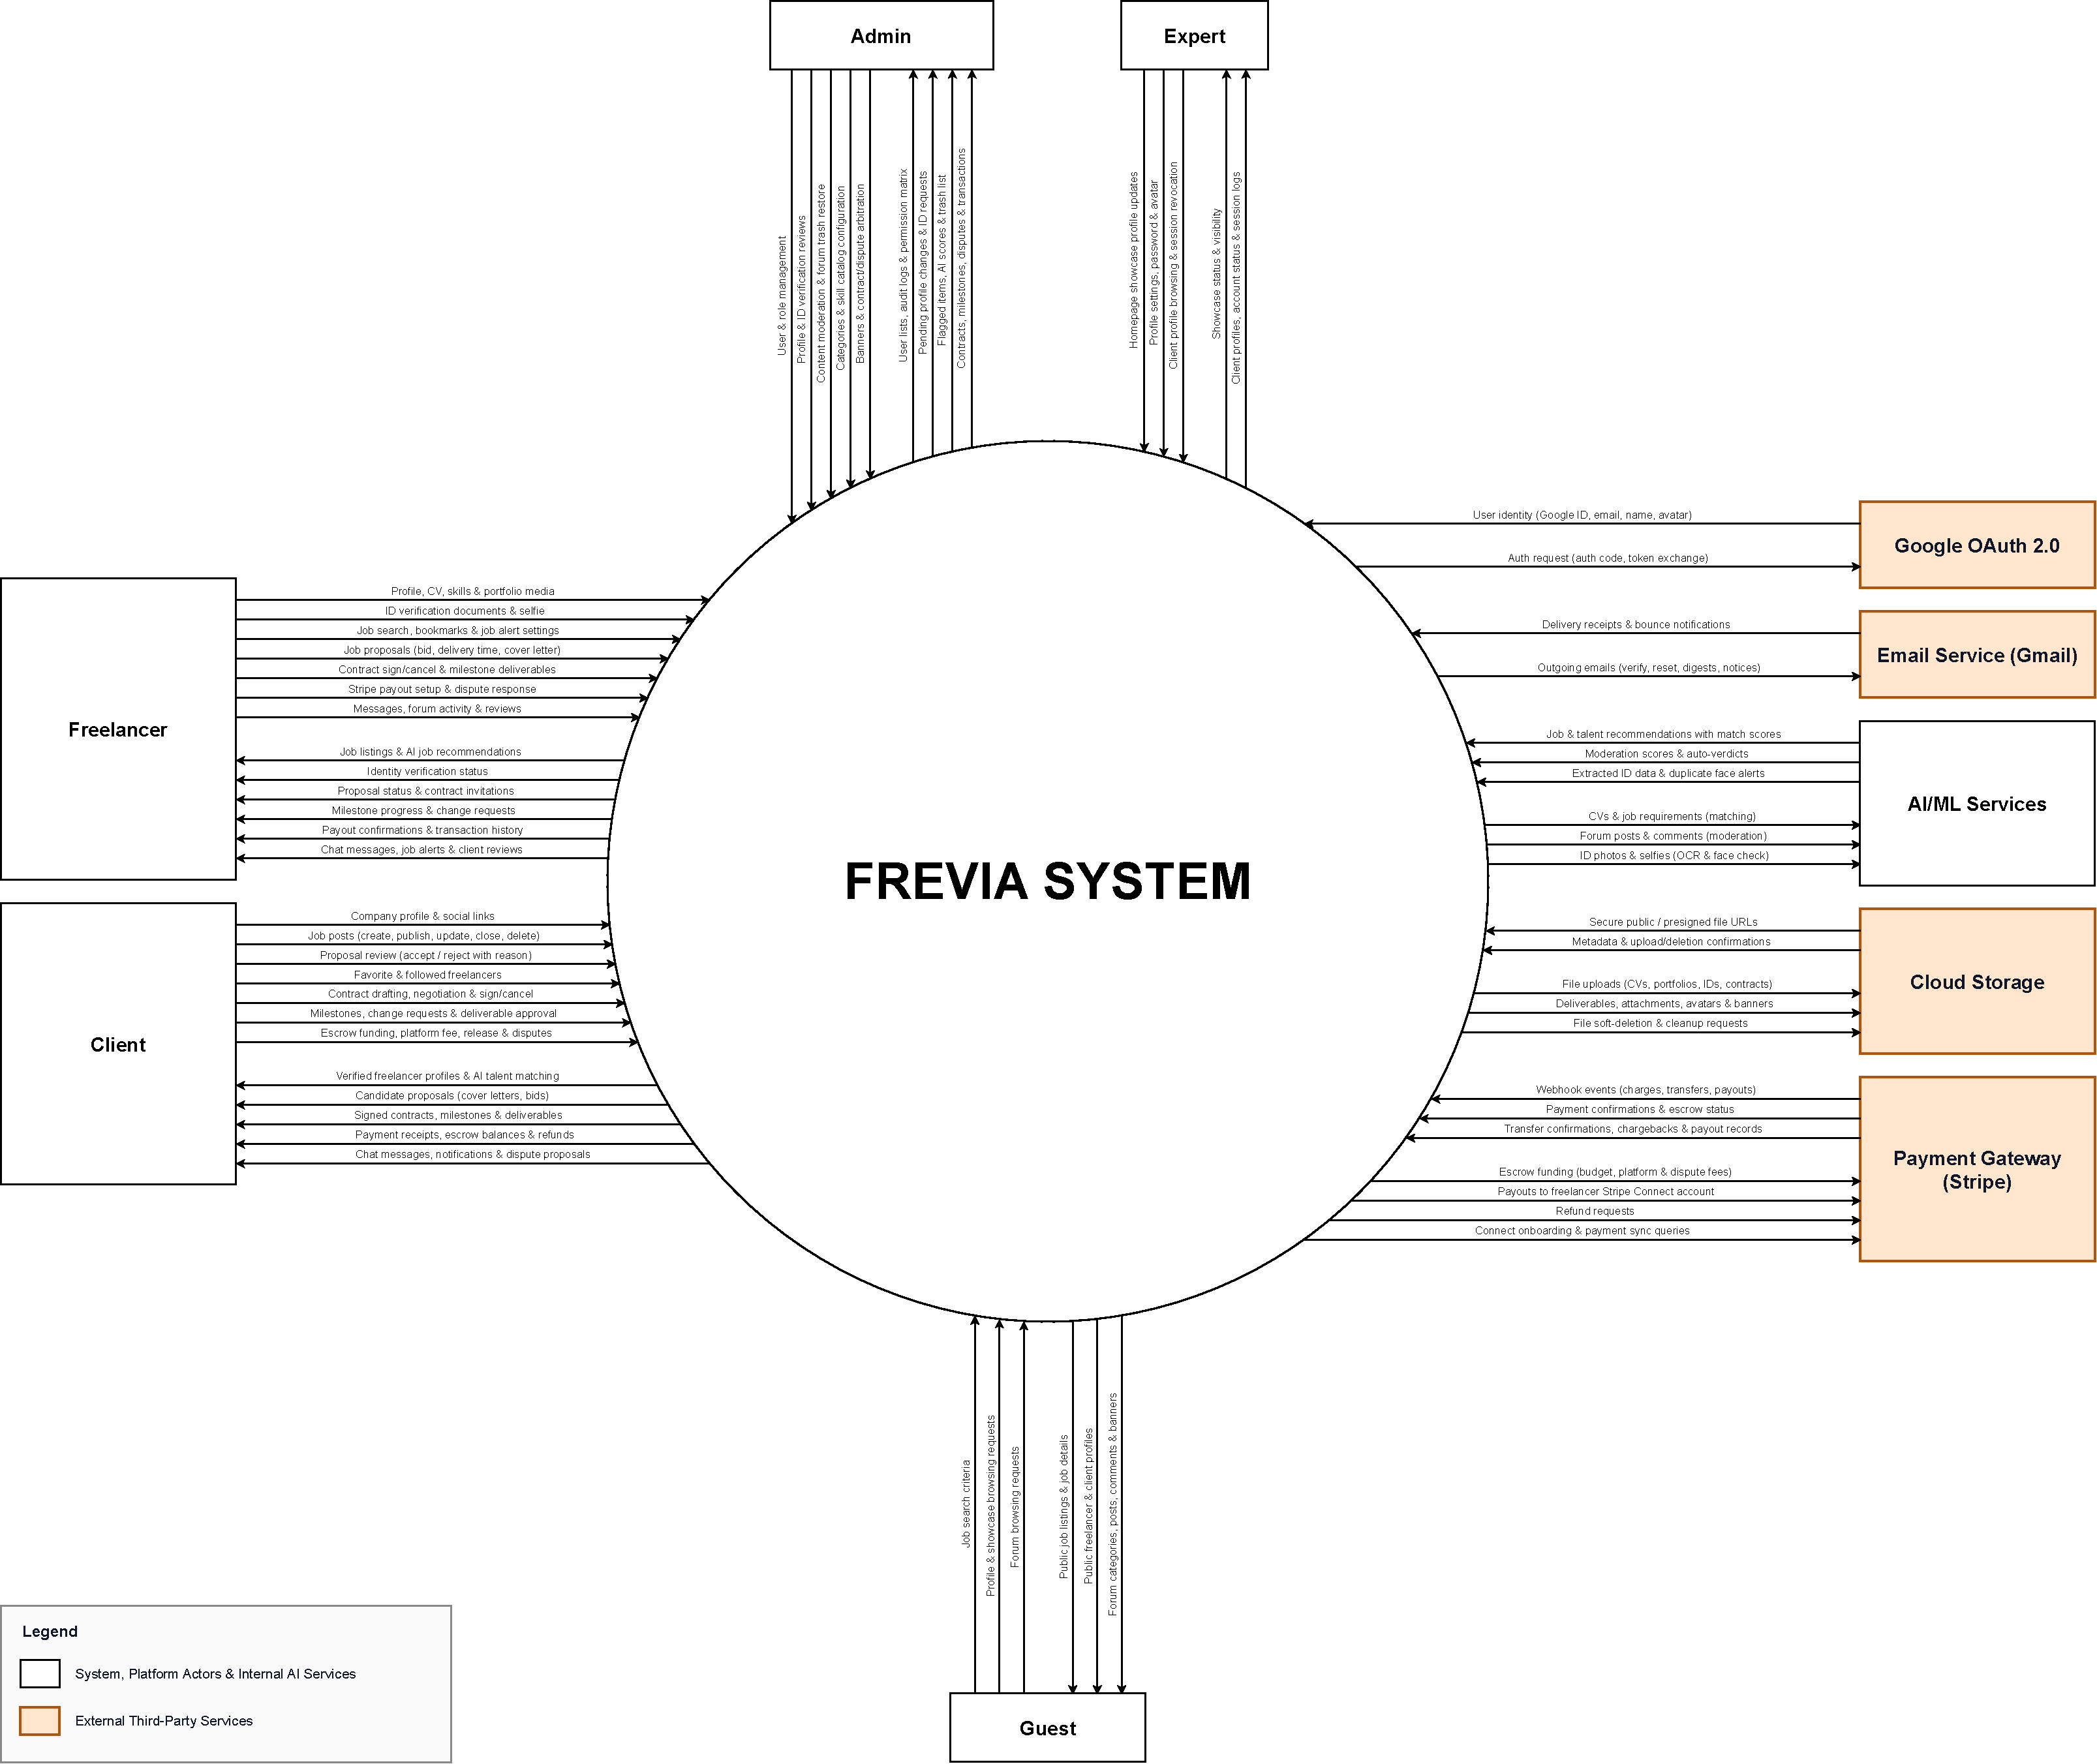
\includegraphics[width=0.82\textwidth, height=0.68\textheight, keepaspectratio]{../Report 3/image/context_diagram/context-diagram.pdf}
  \end{center}
\end{frame}

\begin{frame}[t]{Use Case Diagram -- Client}
  \framesubtitle{Job Posting, AI Candidate Review, Contracting, Milestone Escrow \& Disputes (Report 3)}
  \begin{center}
    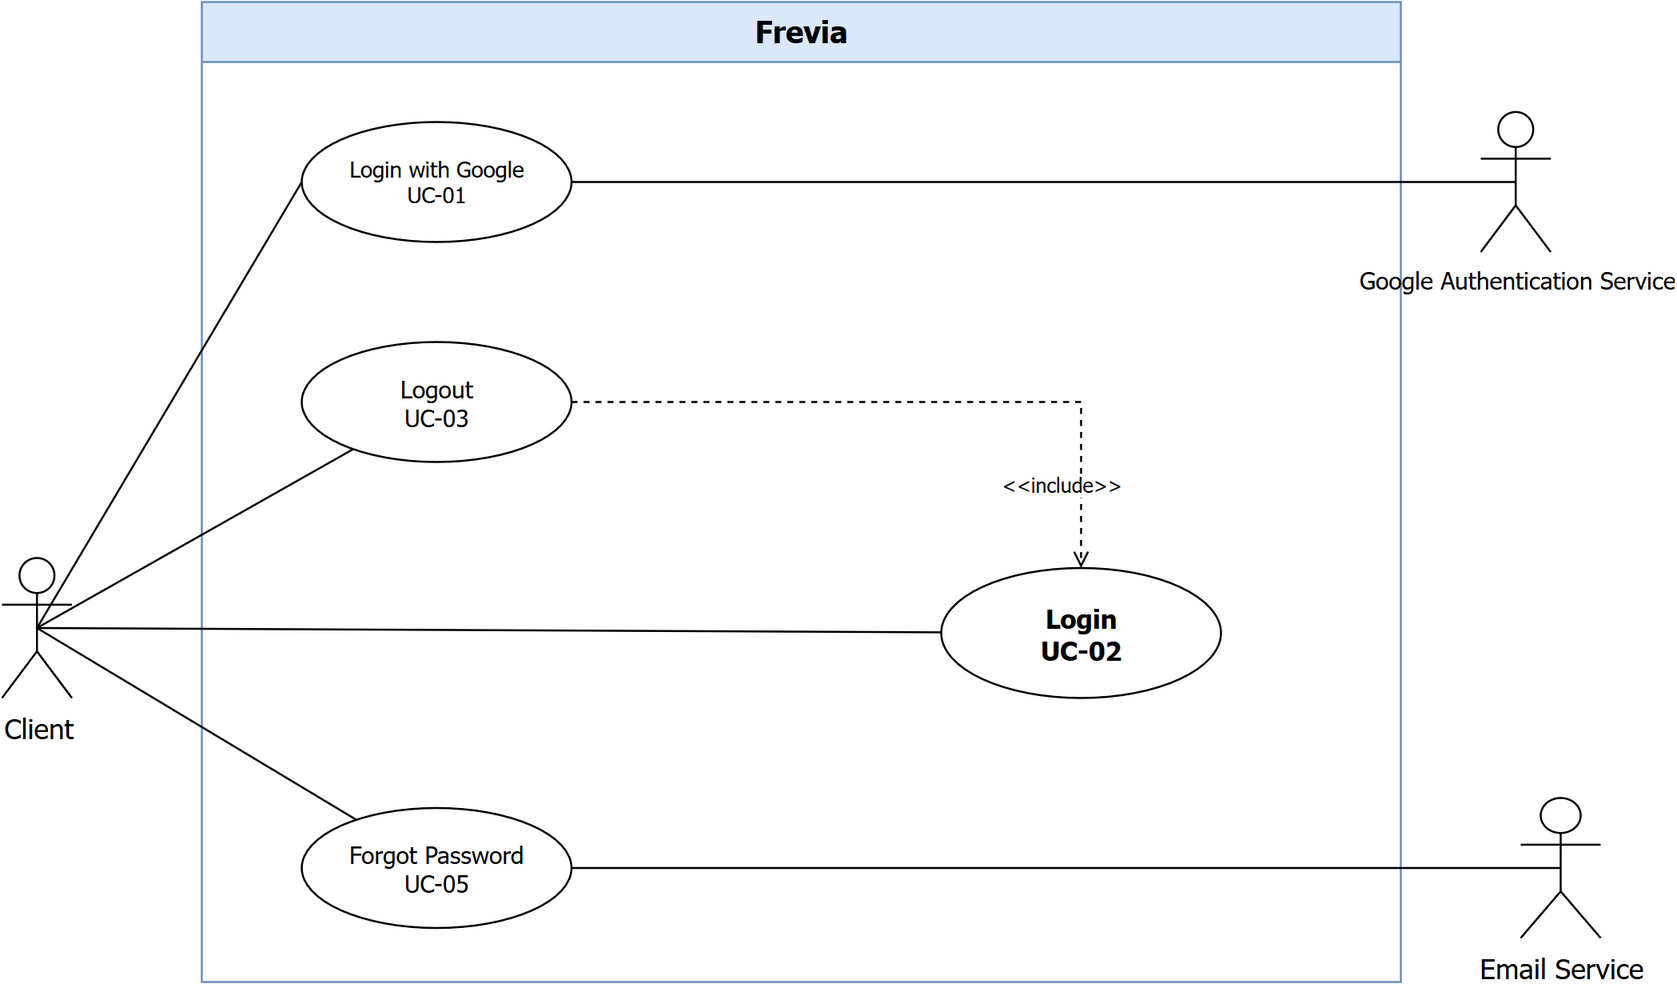
\includegraphics[width=0.90\textwidth, height=0.68\textheight, keepaspectratio]{../Report 3/image/UC_diagram/Client_1.png}
  \end{center}
\end{frame}

\begin{frame}[t]{Use Case Diagram -- Freelancer}
  \framesubtitle{Profile, eKYC Verification, CV Upload, Proposals, Deliverables \& Payouts (Report 3)}
  \begin{center}
    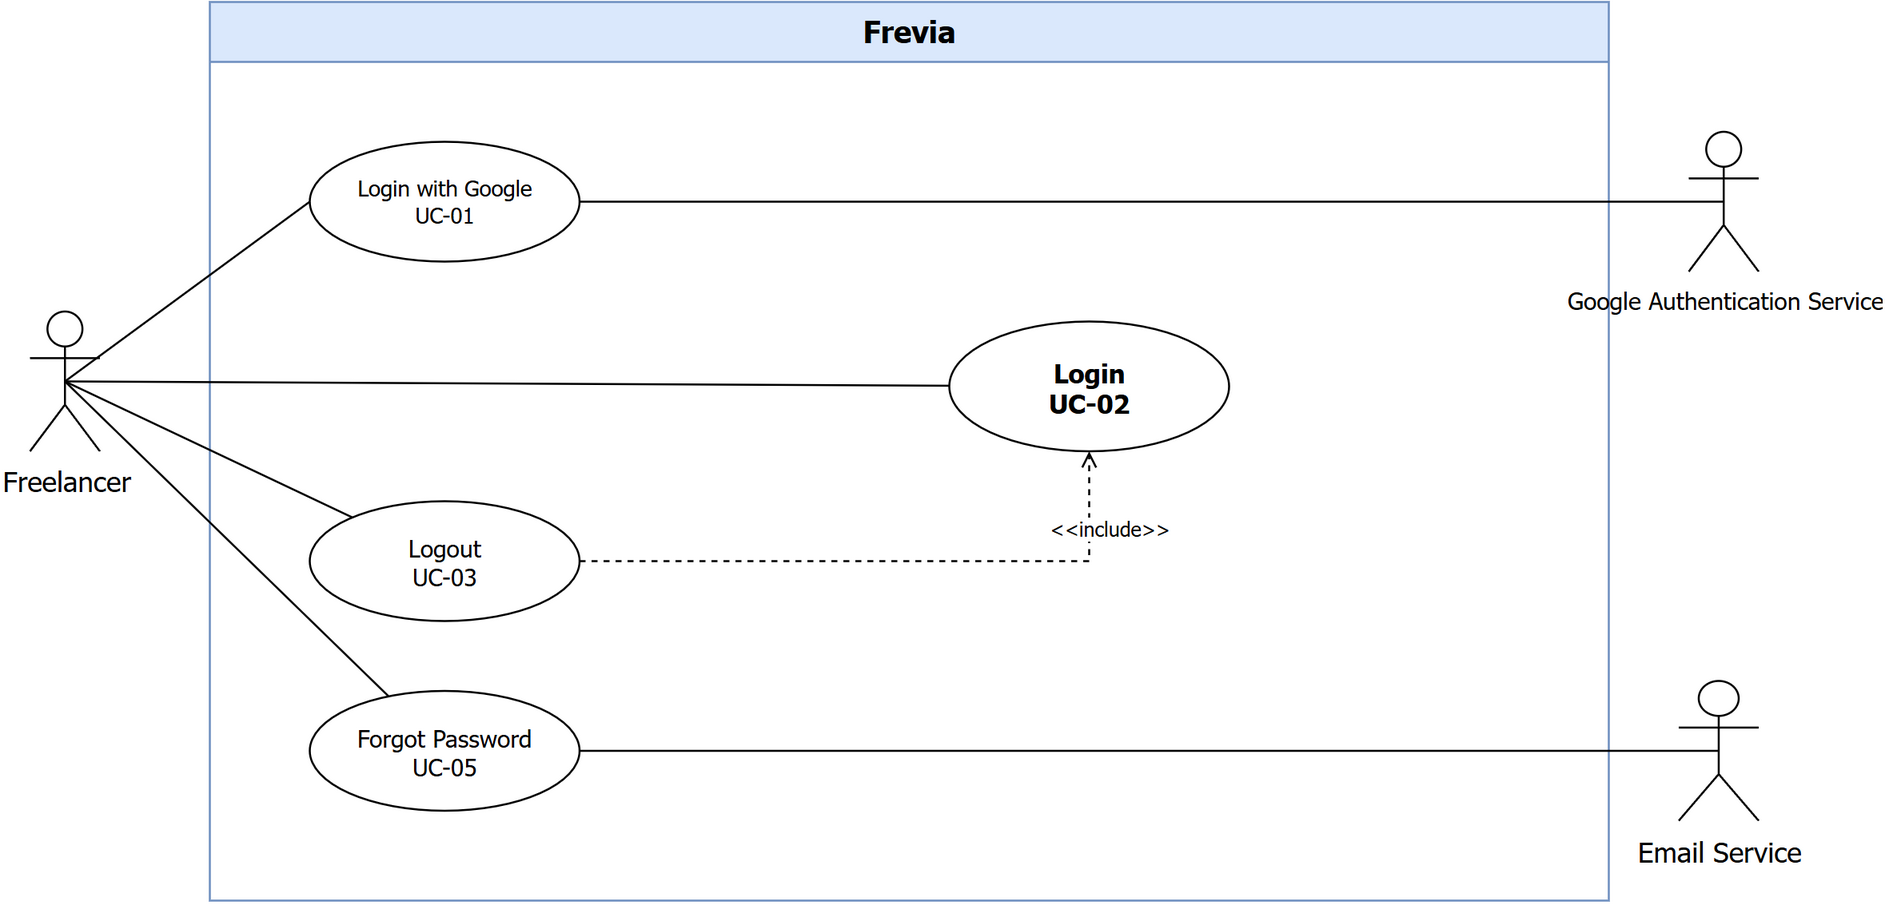
\includegraphics[width=0.90\textwidth, height=0.68\textheight, keepaspectratio]{../Report 3/image/UC_diagram/Freelancer_1.png}
  \end{center}
\end{frame}

\begin{frame}[t]{Use Case Diagram -- Administrator}
  \framesubtitle{User Governance, Dynamic RBAC, eKYC Audit, Moderation \& Catalogs (Report 3)}
  \begin{center}
    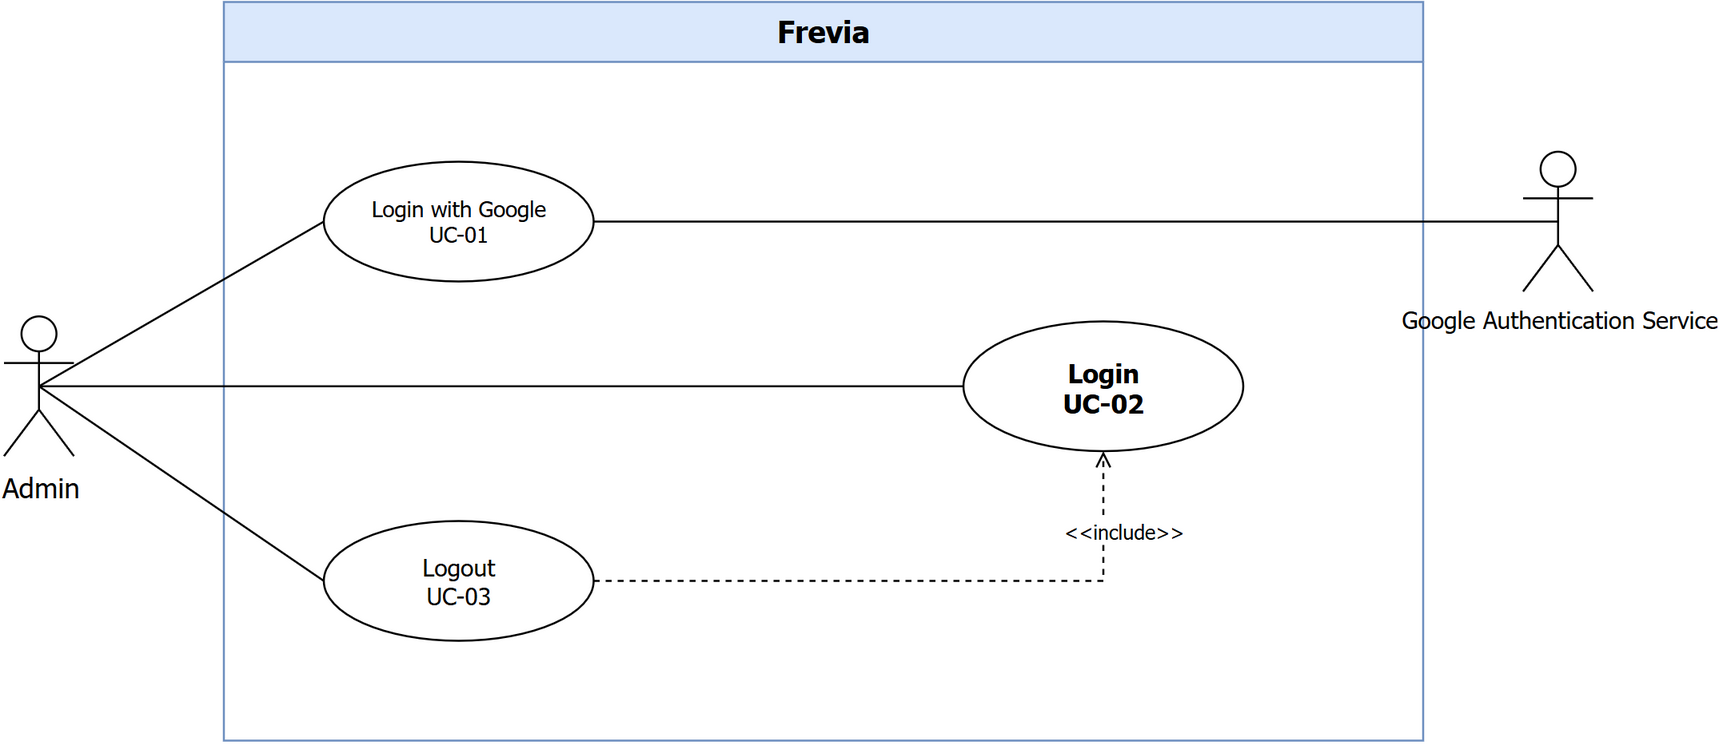
\includegraphics[width=0.90\textwidth, height=0.68\textheight, keepaspectratio]{../Report 3/image/UC_diagram/Admin_1.png}
  \end{center}
\end{frame}

\begin{frame}[t]{Use Case Diagram -- Expert Arbitrator}
  \framesubtitle{Verified Specialist Profile \& Escalated Dispute Arbitration (Report 3)}
  \begin{center}
    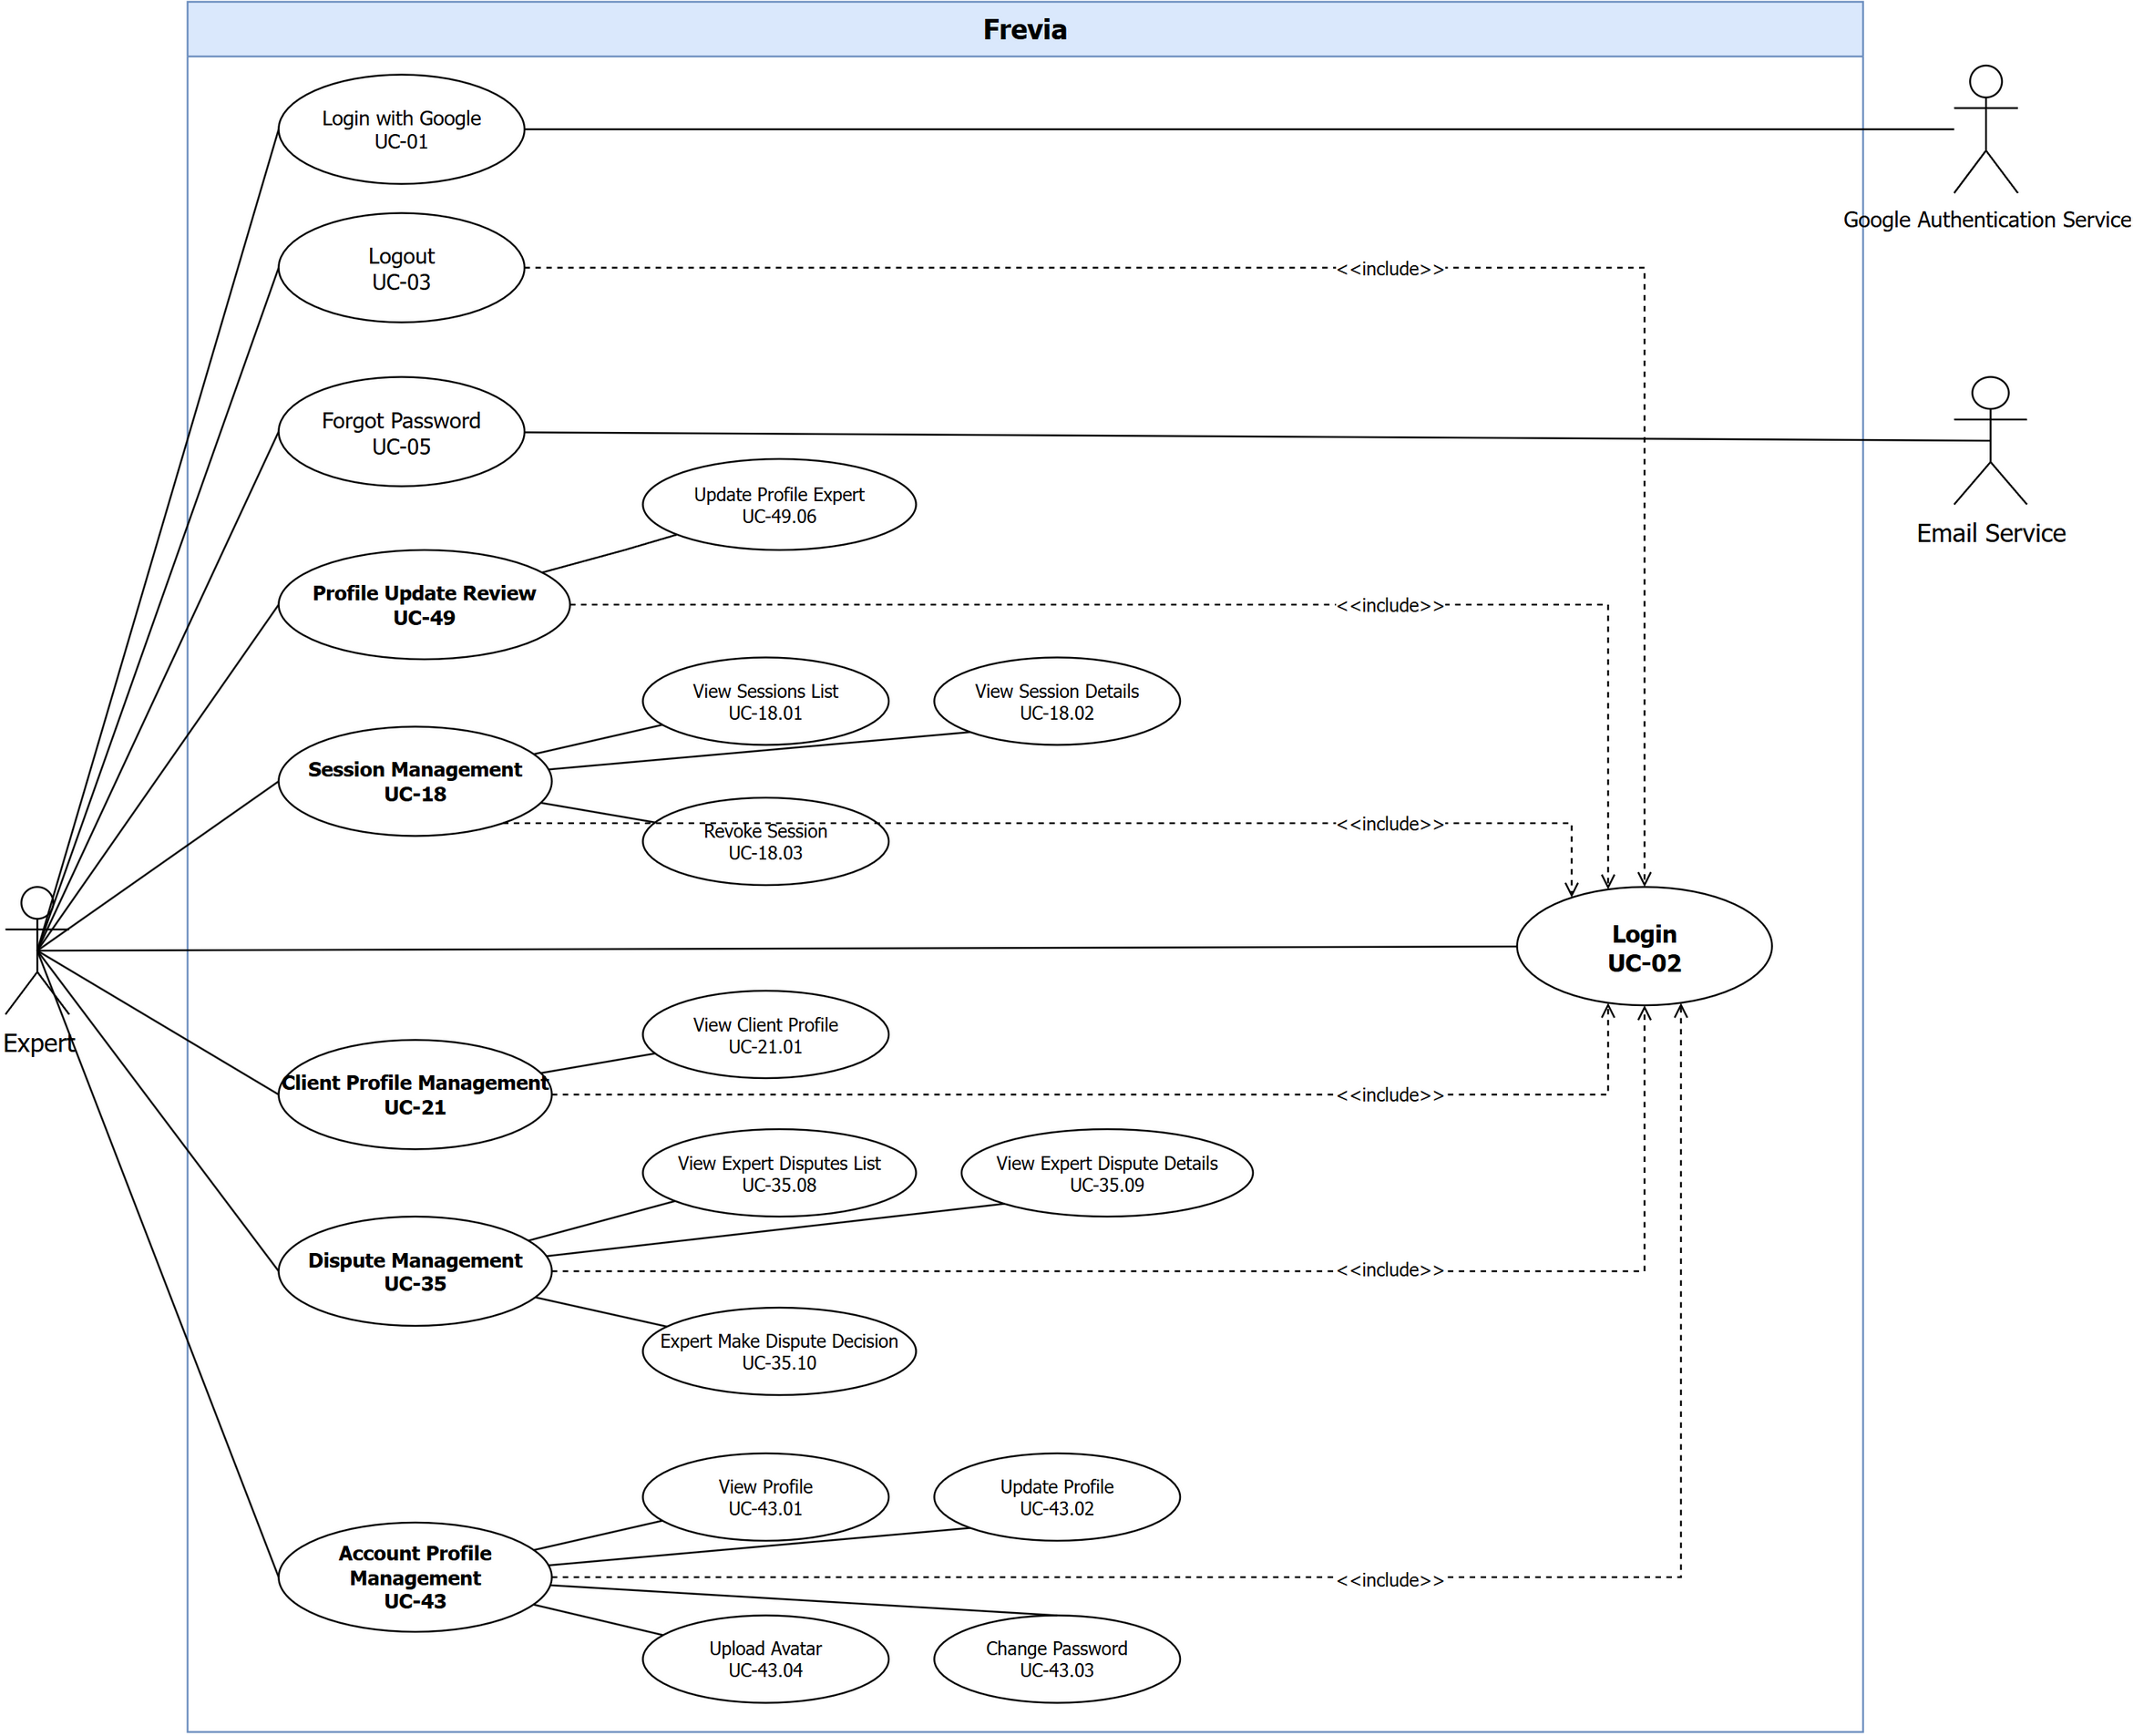
\includegraphics[width=0.90\textwidth, height=0.68\textheight, keepaspectratio]{../Report 3/image/UC_diagram/Expert.png}
  \end{center}
\end{frame}

% ==============================================================================
% CHAPTER IV: SOFTWARE DESIGN
% ==============================================================================
\chapterframe{CHAPTER IV}{Software Design}{N-Layer Architecture, Tech Stack, Database Schema, and AI/Payment Pipelines}

\begin{frame}[t]{Verified Technology Stack}
  \framesubtitle{Derived directly from \texttt{package.json} and \texttt{docker-compose.yml}}
  \begin{columns}[T]
    \begin{column}{0.32\textwidth}
      \cardbox{4.2cm}{Frontend (\texttt{apps/web})}{%
        \bul{Next.js \textbf{16.2.0}} (App Router)\\[3pt]
        \bul{React \textbf{19.2.0}}, TS \textbf{5.9.2}\\[3pt]
        \bul{TailwindCSS \textbf{4.3.2}} + shadcn/ui\\[3pt]
        \bul{TanStack Query \textbf{5.101}}\\[3pt]
        \bul{Zod \textbf{4.4.3}} + React Hook Form\\[3pt]
        \bul{\texttt{next-intl} (\texttt{en}/\texttt{vi}), Tiptap \textbf{3.28}}
      }
    \end{column}
    \begin{column}{0.32\textwidth}
      \cardbox{4.2cm}{Backend (\texttt{apps/api})}{%
        \bul{NestJS \textbf{11.0.1}} (33 modules)\\[2pt]
        \bul{Prisma \textbf{7.8.0}} + PostgreSQL \textbf{16} (71 models)\\[2pt]
        \bul{Socket.IO \textbf{11.2.1}} (WebSockets)\\[2pt]
        \bul{JWT + Google OAuth 2.0}\\[2pt]
        \bul{Stripe, Cloudinary, Nodemailer}
      }
    \end{column}
    \begin{column}{0.32\textwidth}
      \cardbox{4.2cm}{AI \& Infrastructure}{%
        \bul{\textbf{eKYC (8001):} RapidOCR, UltraFace, ArcFace (ONNX), MediaPipe}\\[3pt]
        \bul{\textbf{CV Match (8000):} BGE-M3, ChromaDB, Ollama (\texttt{qwen3:4b})}\\[3pt]
        \bul{\textbf{Moderation (8002):} Optional HTTP service w/ safe fallback}\\[3pt]
        \bul{pnpm 9, Turborepo, Infisical, Docker}
      }
    \end{column}
  \end{columns}
\end{frame}

\begin{frame}[t]{System Architecture (N-Layer + AI Microservices)}
  \framesubtitle{Client, Presentation, Business Logic (33 Modules), Data Access, Shared Libs \& AI}
  \begin{center}
    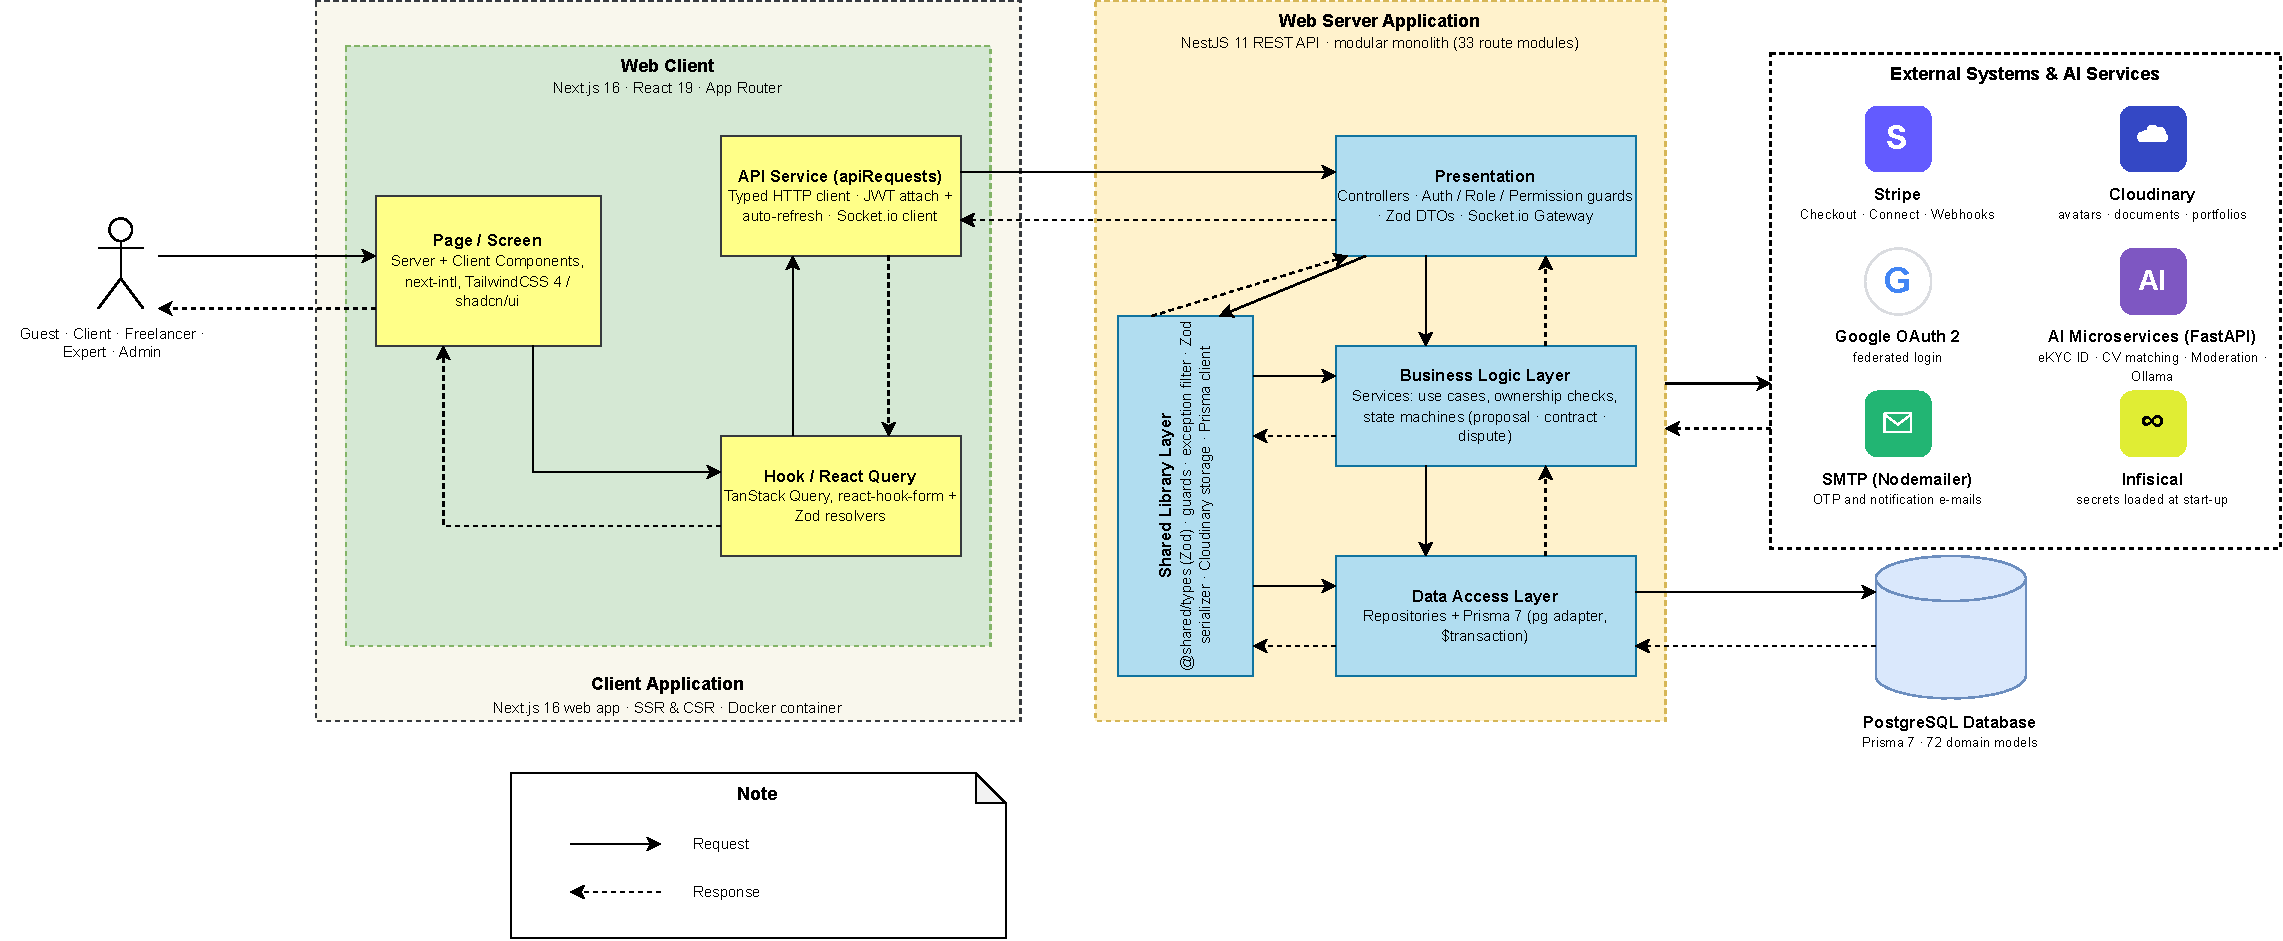
\includegraphics[width=0.92\textwidth, height=0.73\textheight, keepaspectratio]{../Report 4/images/architecture/frevia-overall-architecture.pdf}
  \end{center}
\end{frame}

\begin{frame}[t]{Monorepo Package Architecture}
  \framesubtitle{pnpm Workspaces + Turborepo: Strict downward dependencies \& module isolation}
  \begin{center}
    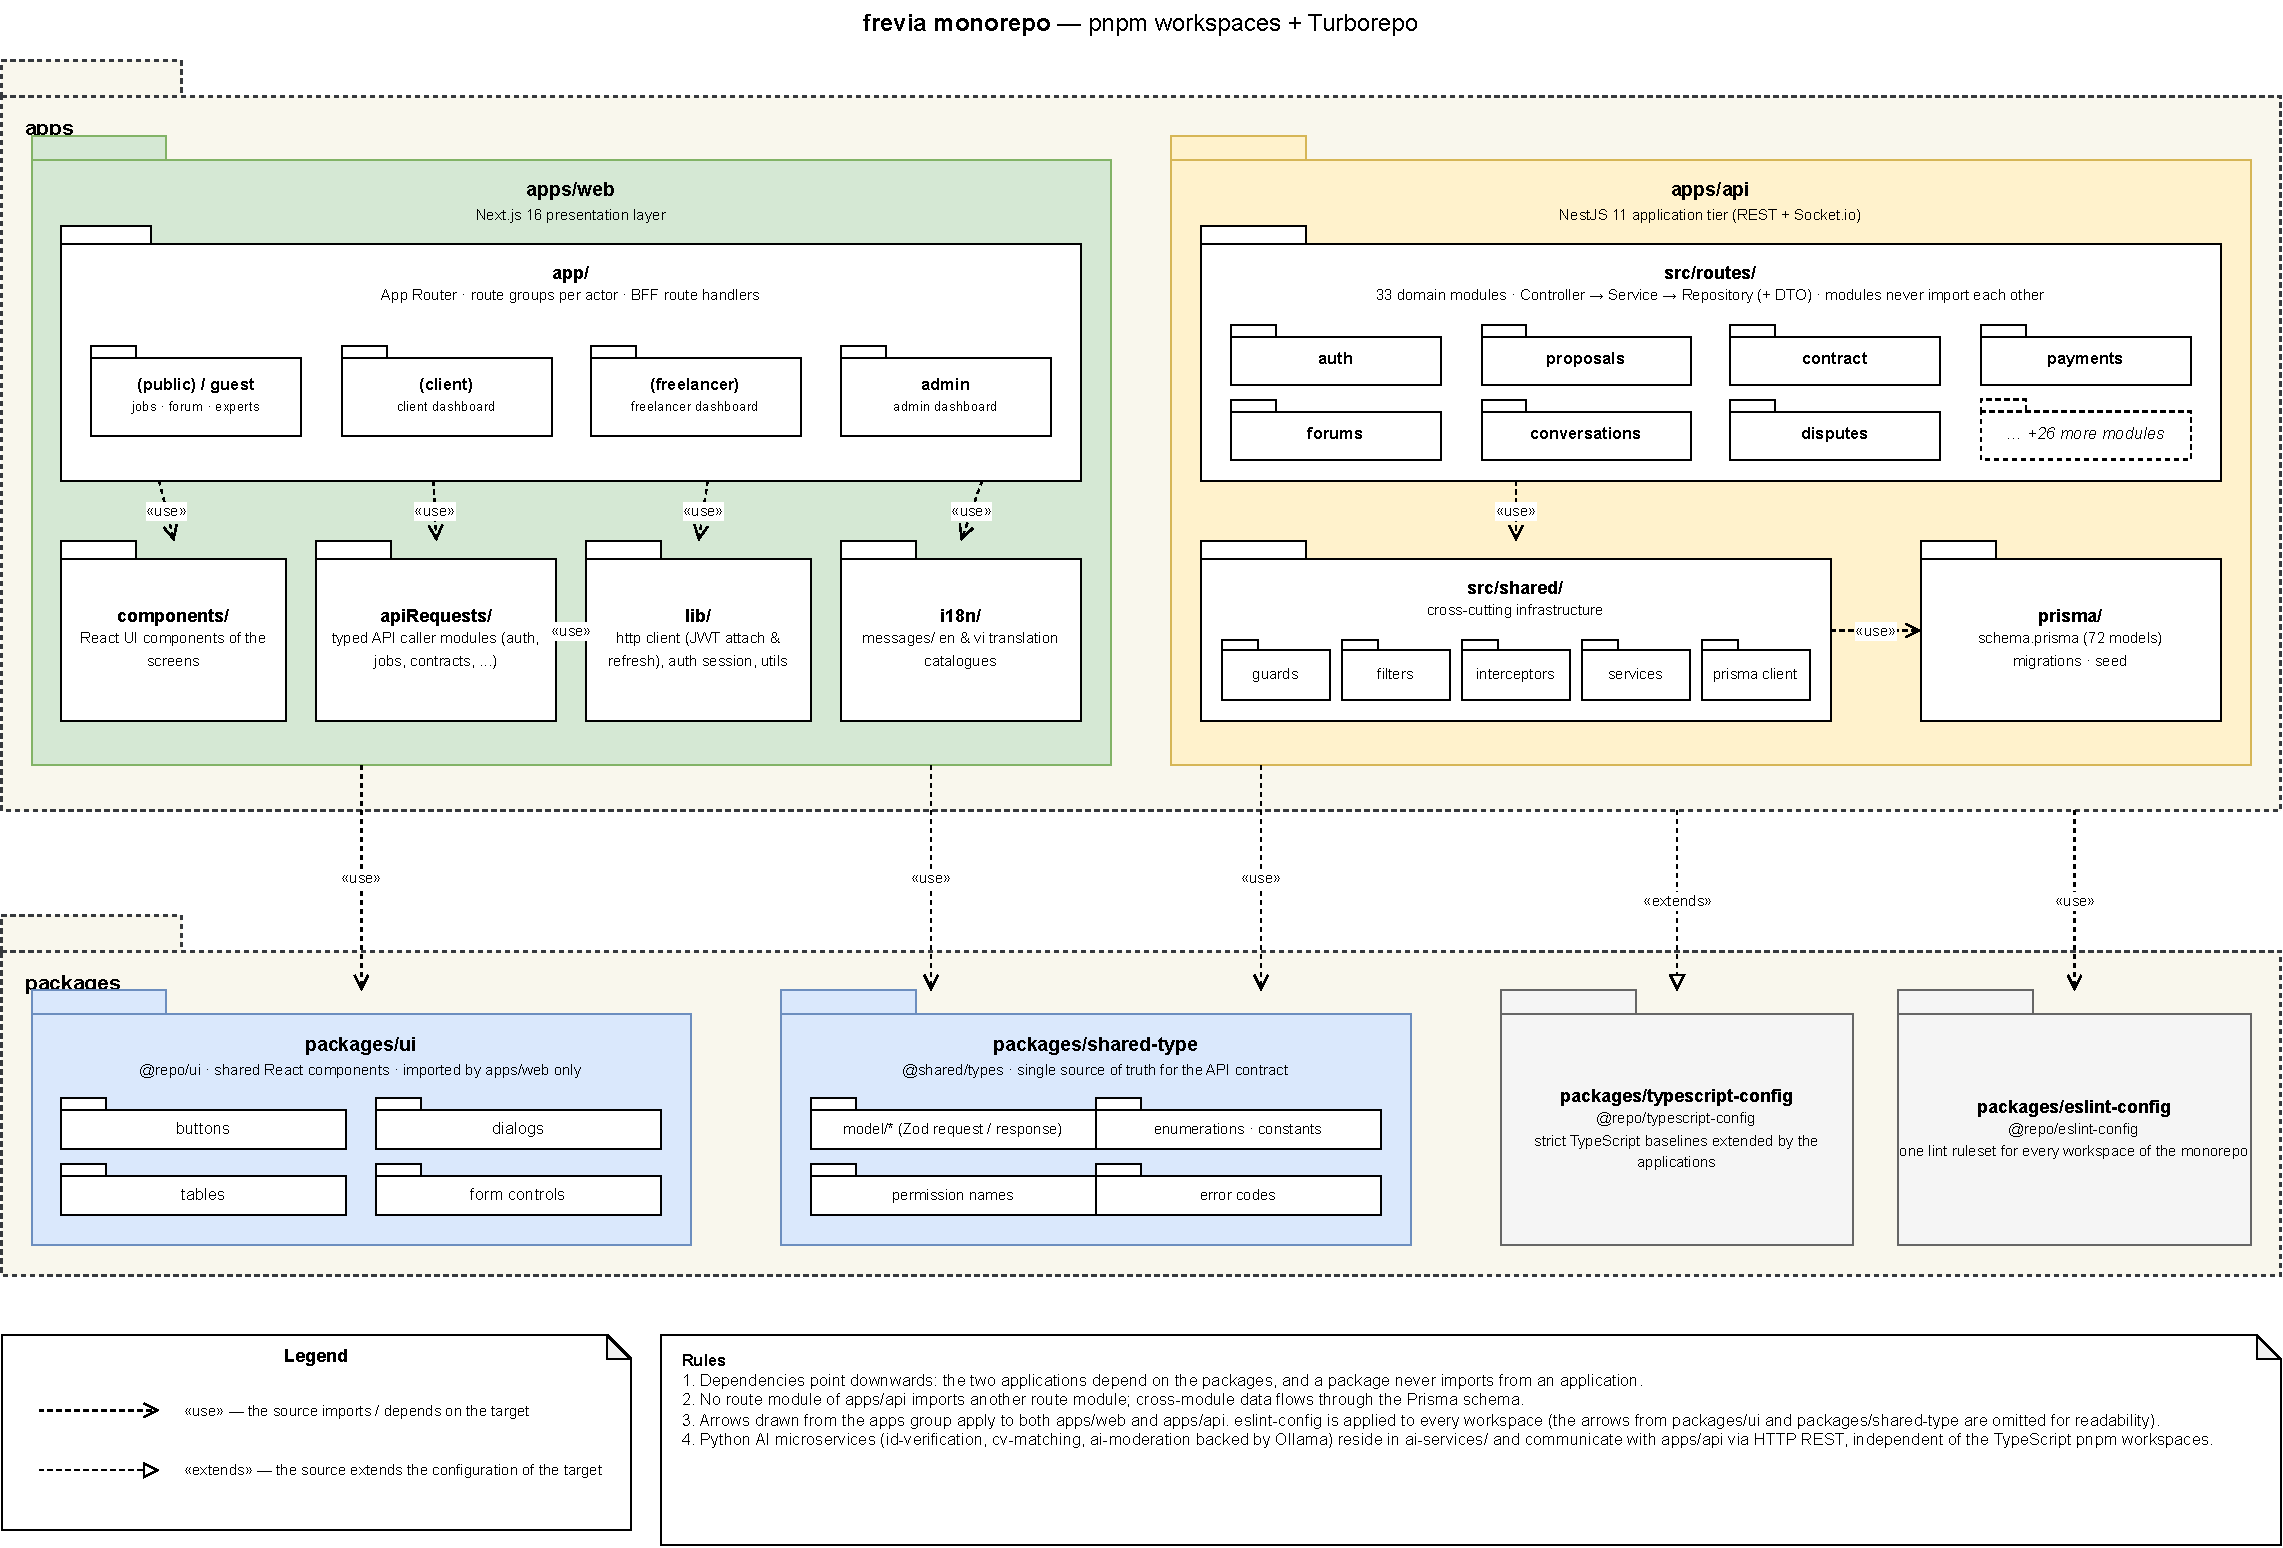
\includegraphics[width=0.90\textwidth, height=0.68\textheight, keepaspectratio]{../Report 4/images/architecture/frevia-package-diagram.pdf}
  \end{center}
\end{frame}

\begin{frame}[t]{Database Architecture -- Overall Schema}
  \framesubtitle{PostgreSQL 16 + Prisma 7 ORM -- Full System Schema (71 Models, 43 Enums)}
  \begin{center}
    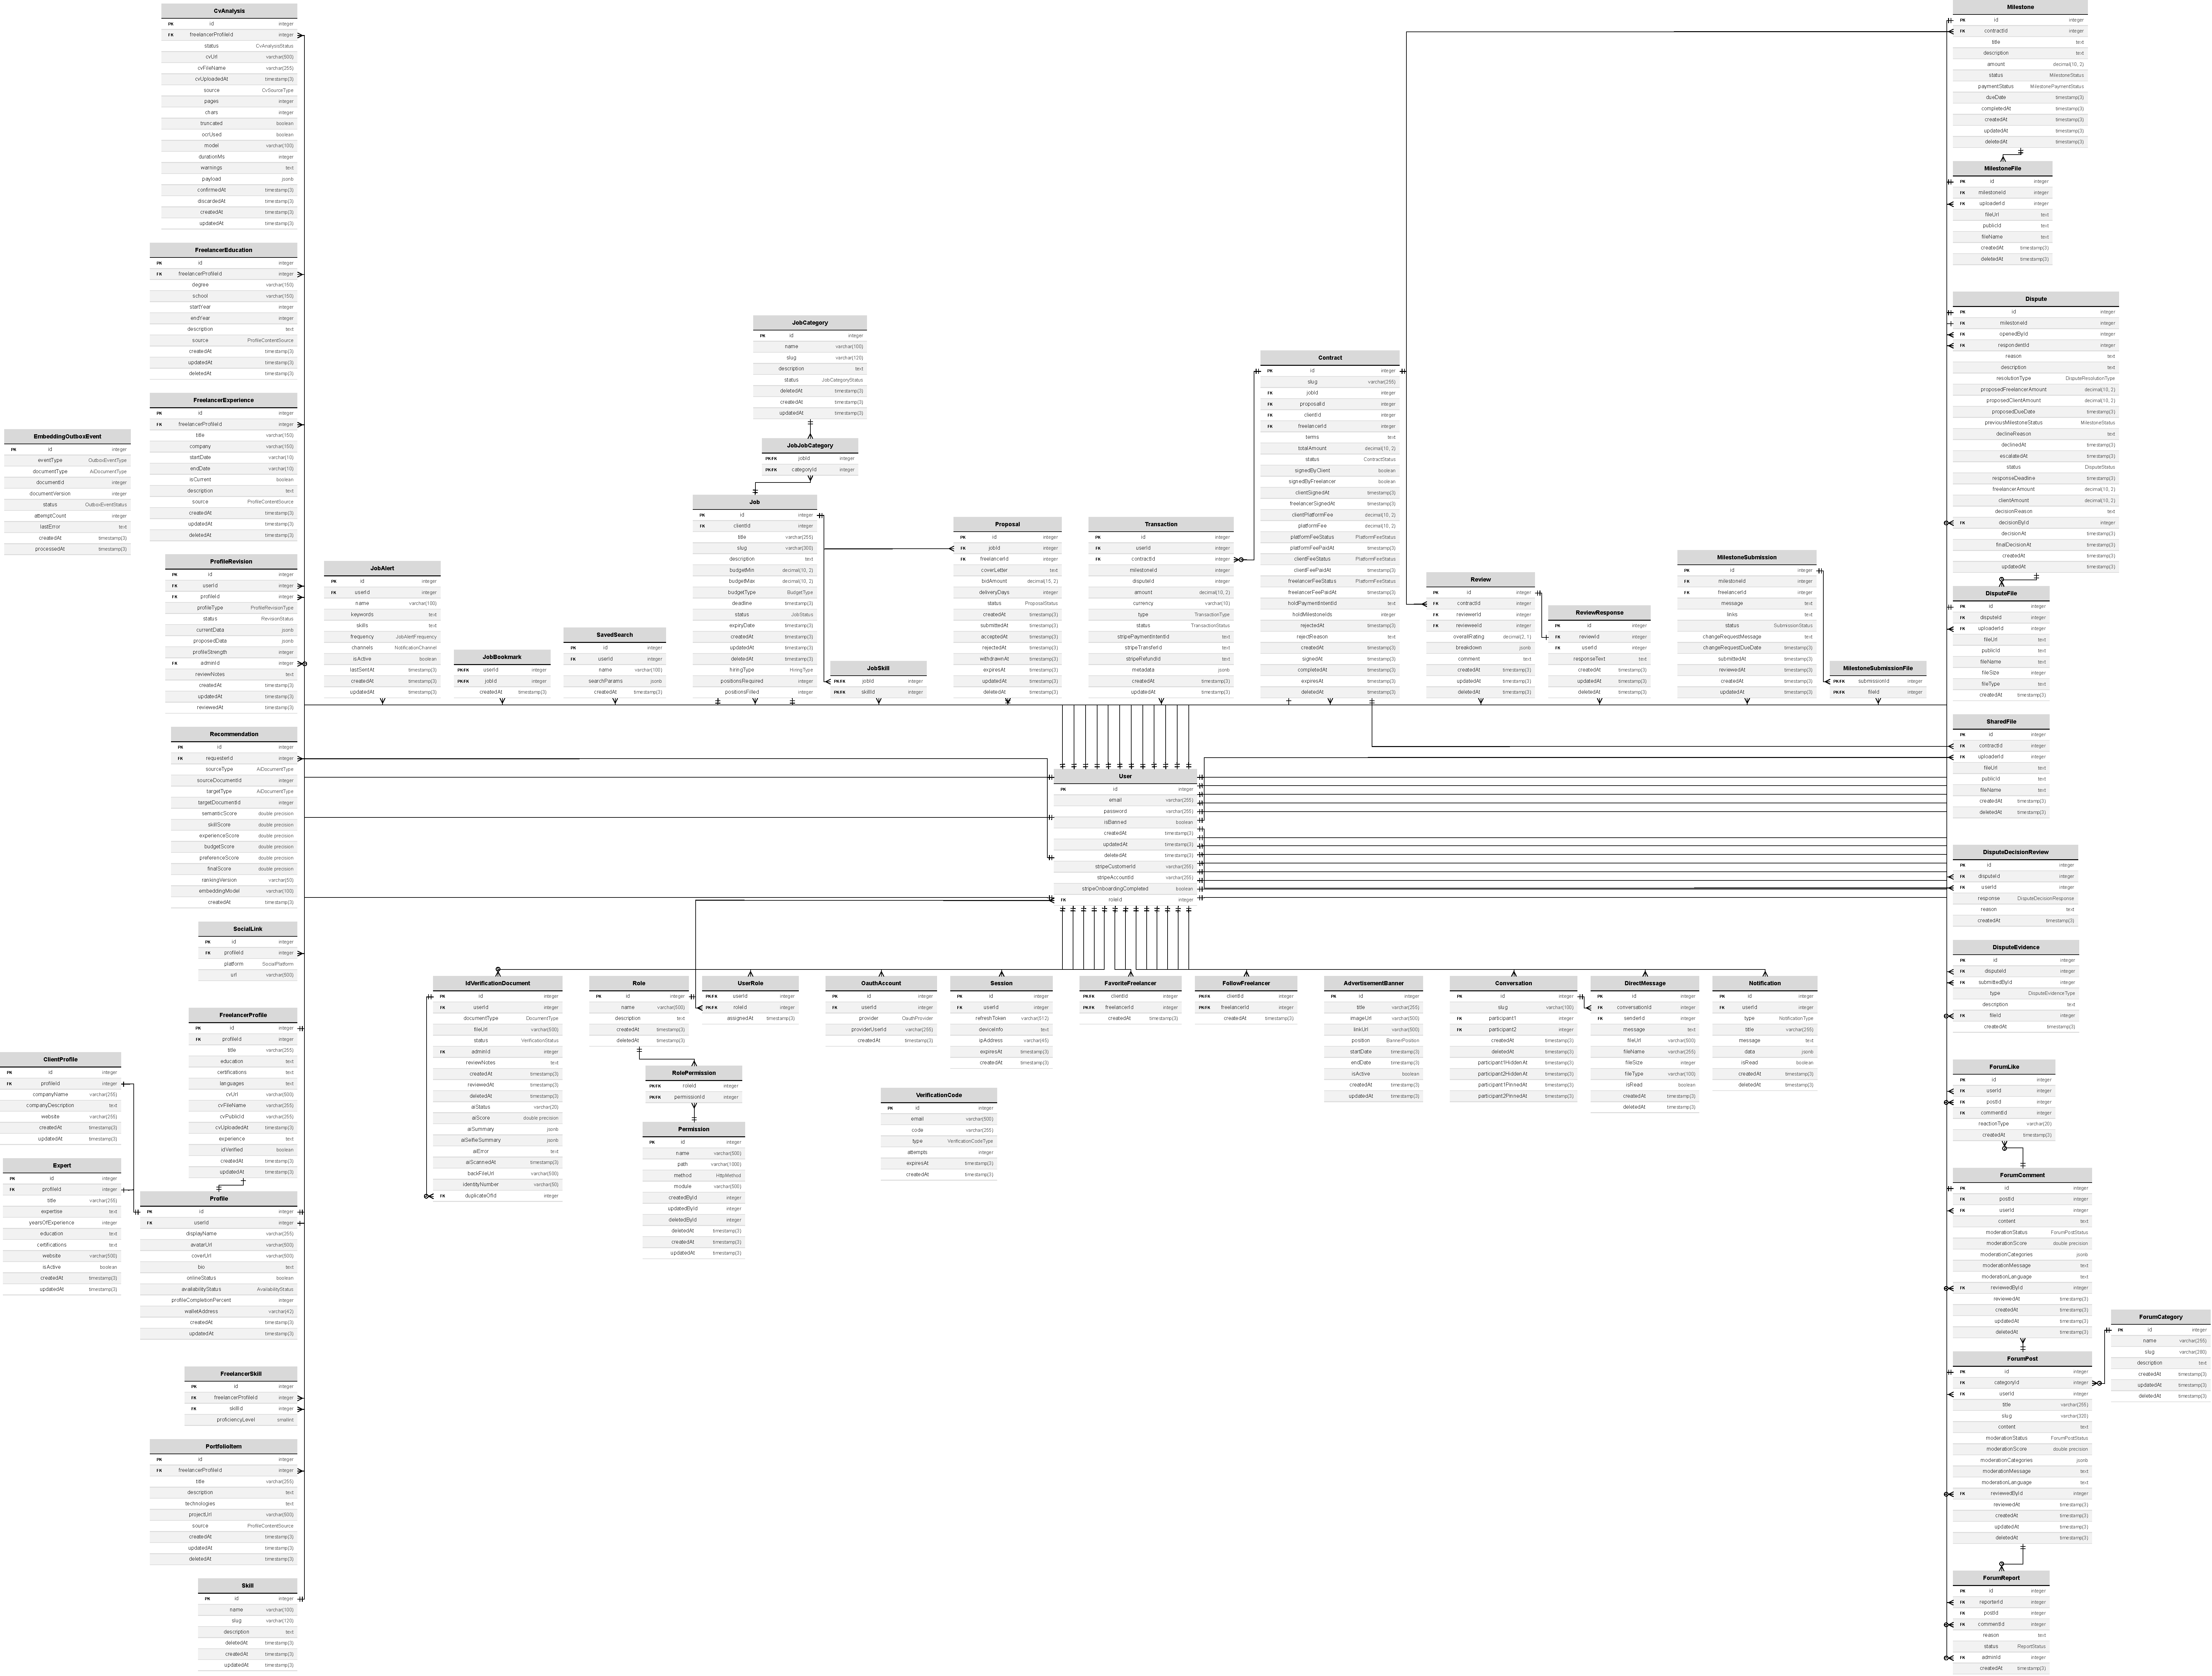
\includegraphics[width=0.92\textwidth, height=0.68\textheight, keepaspectratio]{../Report 4/images/database/erd.pdf}
  \end{center}
\end{frame}

\begin{frame}[t]{Core DB -- Contract Schema (ERD11)}
  \framesubtitle{Links Job, Proposal, Client, Freelancer, Milestones \& Dual-Signature State (Report 4)}
  \begin{center}
    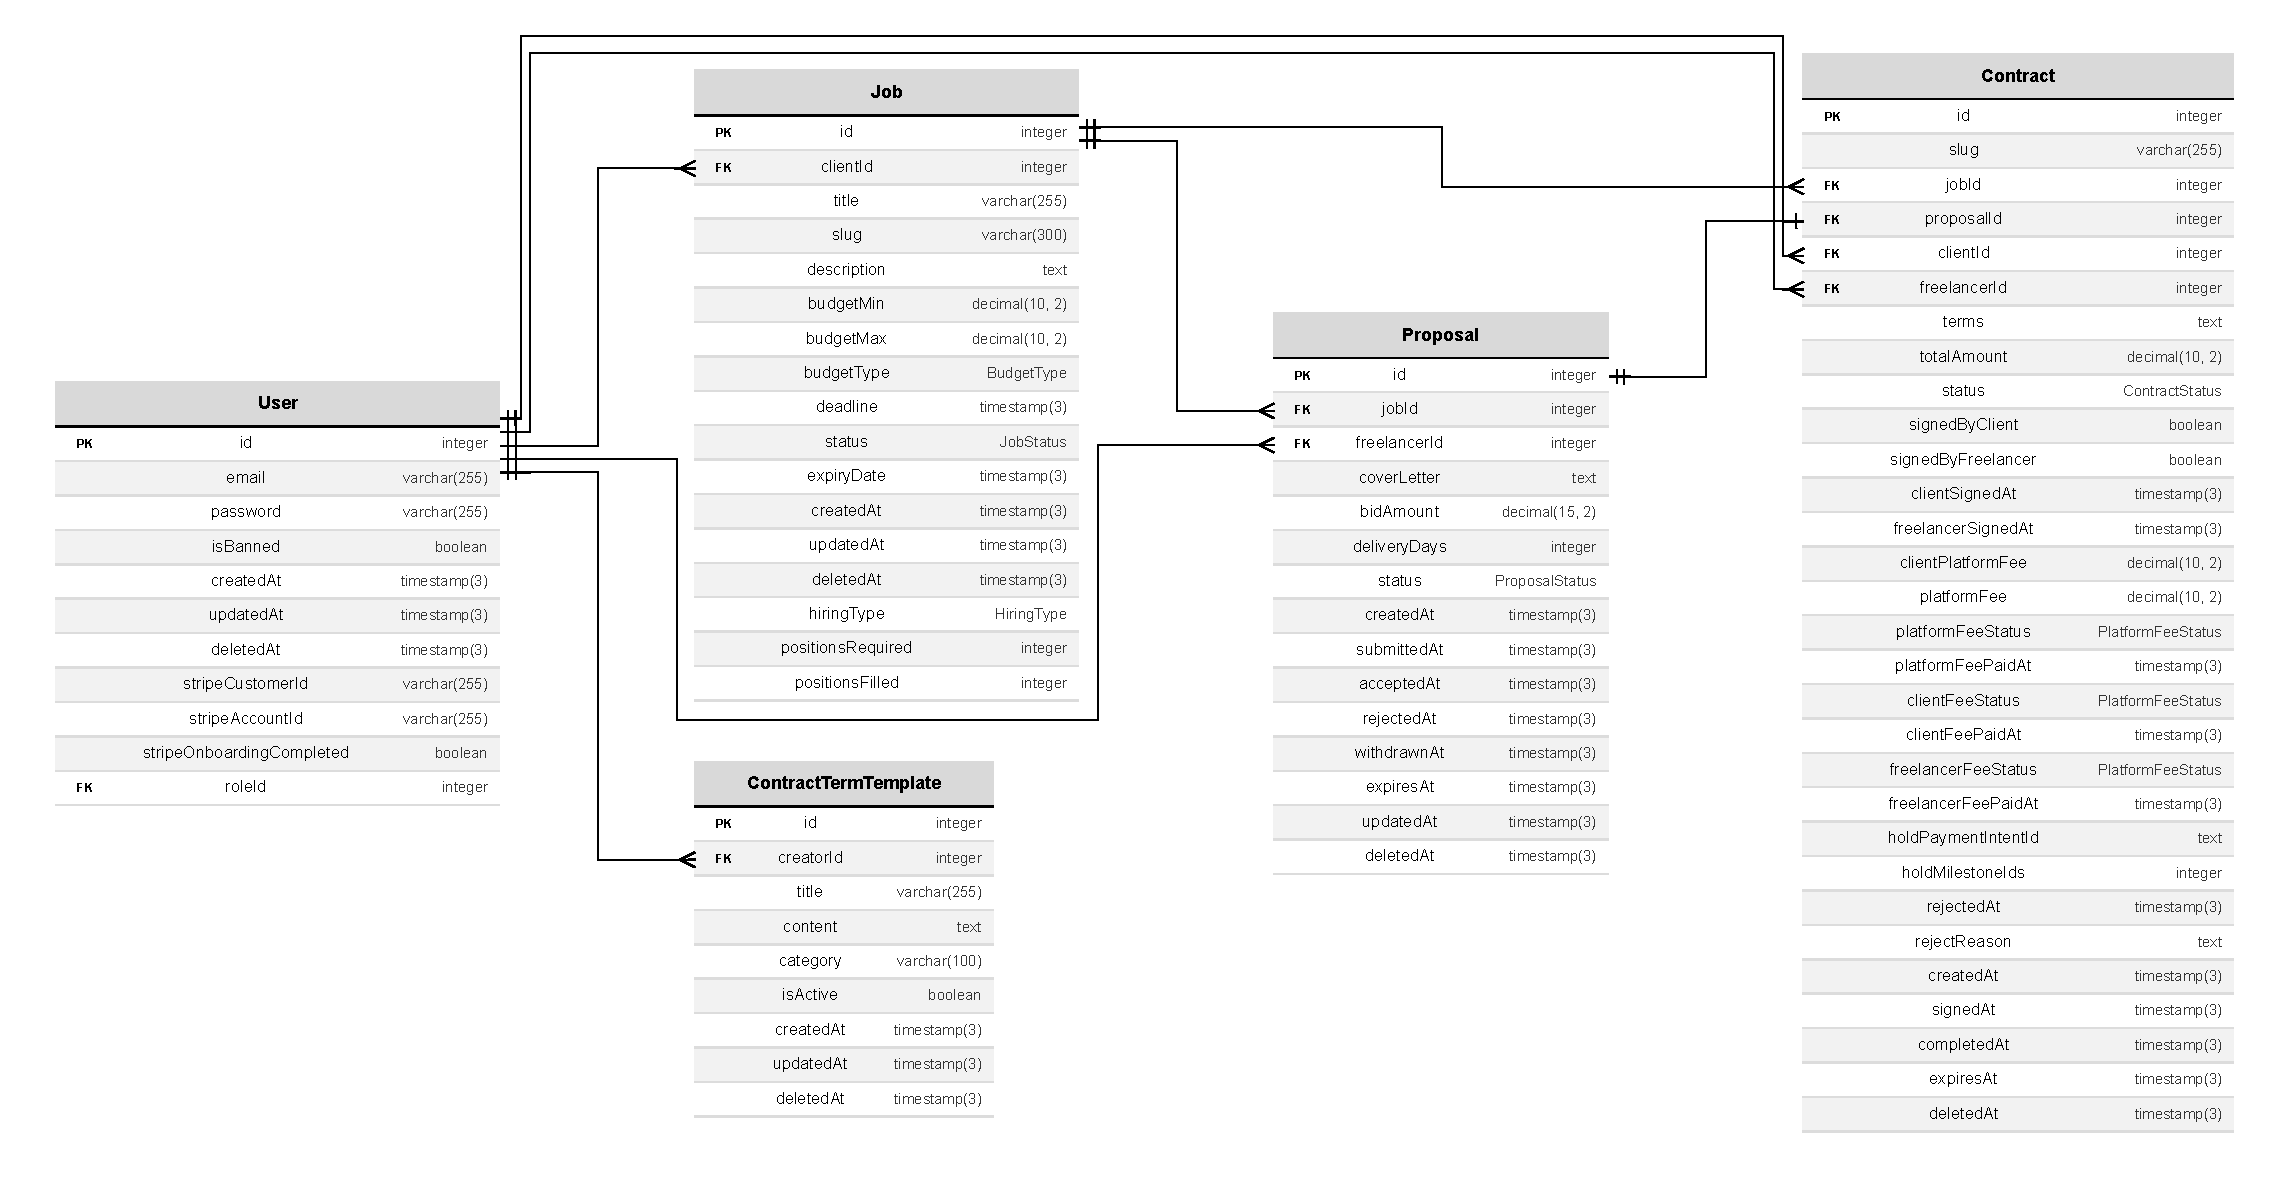
\includegraphics[width=0.90\textwidth, height=0.66\textheight, keepaspectratio]{../Report 4/images/database/erd-11.pdf}
  \end{center}
\end{frame}

\begin{frame}[t]{Core DB -- Escrow \& Payments (ERD14)}
  \framesubtitle{Milestone Escrow Funding, Stripe Transfers, Transactions \& Certificates (Report 4)}
  \begin{center}
    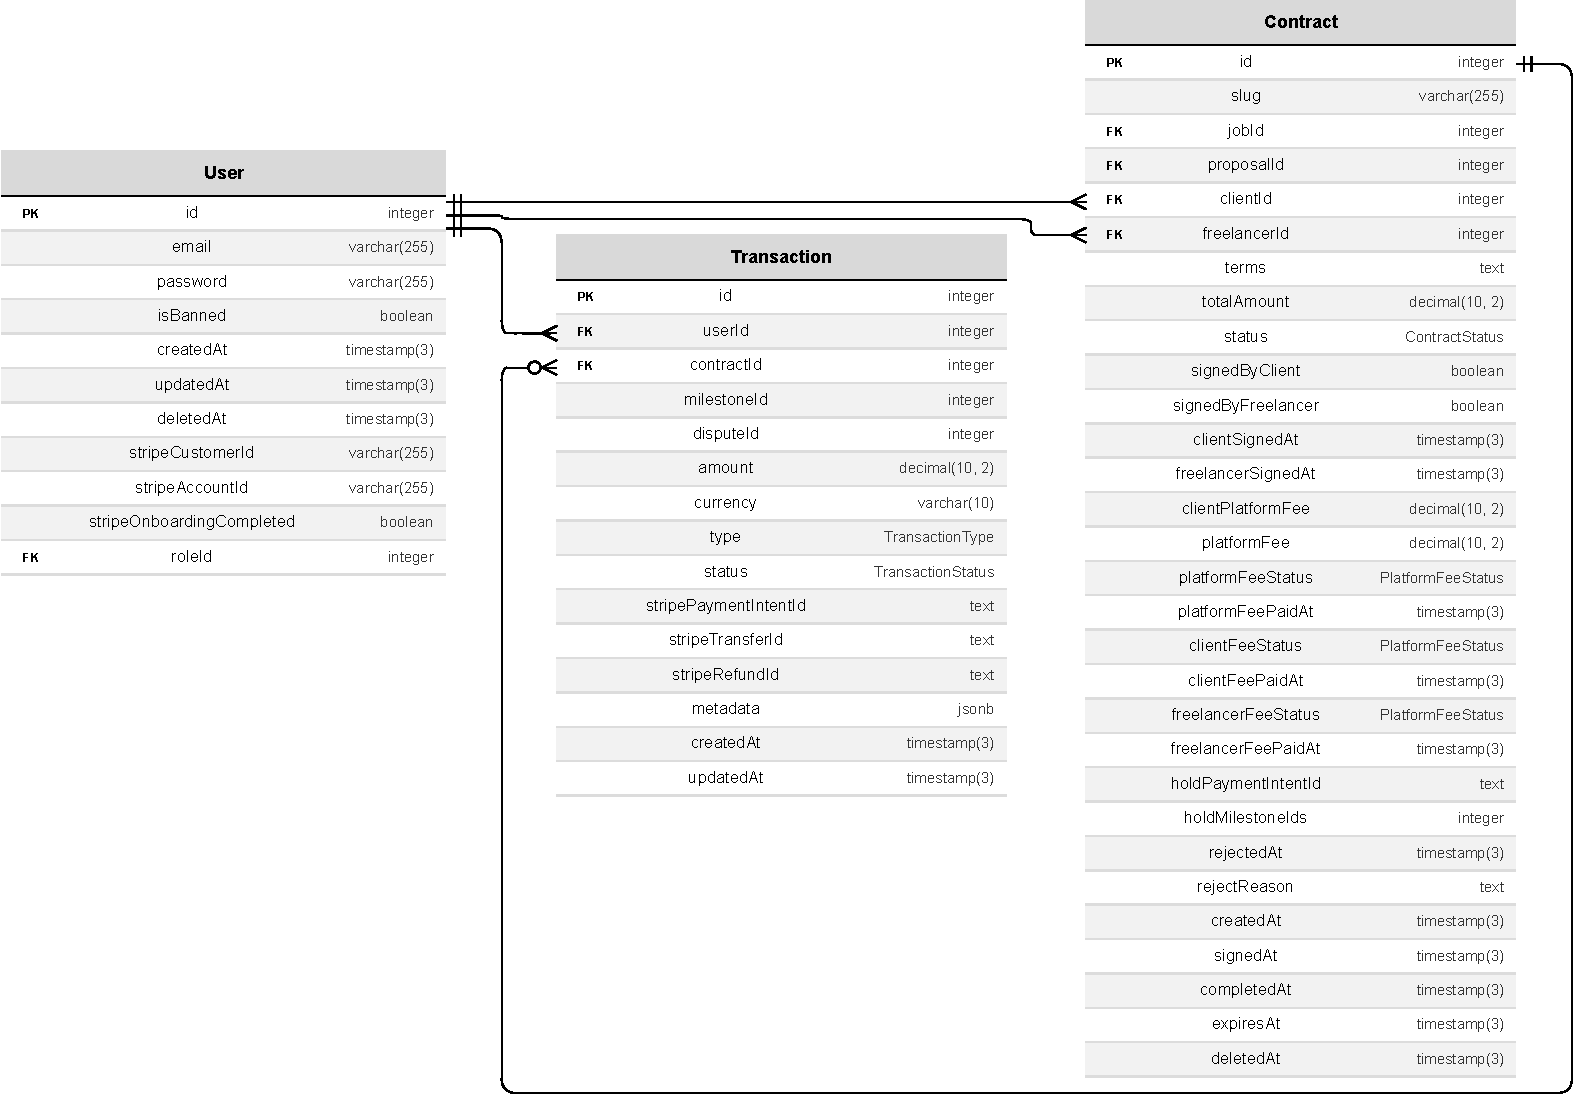
\includegraphics[width=0.90\textwidth, height=0.66\textheight, keepaspectratio]{../Report 4/images/database/erd-14.pdf}
  \end{center}
\end{frame}

\begin{frame}[t]{Core Business Flow \& State Machine Safeguards}
  \framesubtitle{End-to-End Verified Contracting \& Escrow Lifecycle}
  \vspace{2pt}
  \begin{center}
  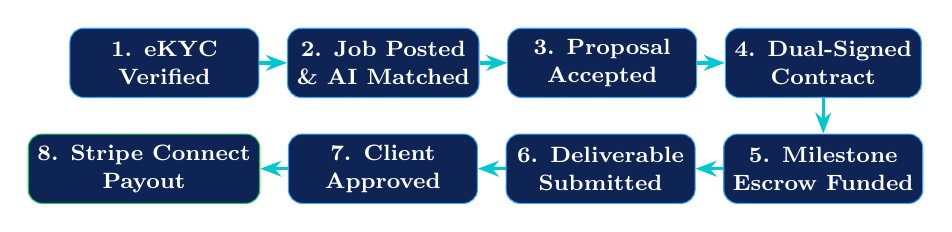
\begin{tikzpicture}[
    node distance=0.35cm and 0.35cm,
    stepbox/.style={draw=fptaccent, fill=fptcard, rounded corners=5pt, minimum width=2.4cm, minimum height=0.88cm,
                    align=center, font=\fontsize{8.3}{10}\selectfont\bfseries, text=white},
    arr/.style={-{Stealth[scale=0.9]}, fptteal, line width=1.2pt}
  ]
    \node[stepbox] (s1) {1. eKYC\\Verified};
    \node[stepbox, right=of s1] (s2) {2. Job Posted\\\& AI Matched};
    \node[stepbox, right=of s2] (s3) {3. Proposal\\Accepted};
    \node[stepbox, right=of s3] (s4) {4. Dual-Signed\\Contract};
    \node[stepbox, below=0.45cm of s4] (s5) {5. Milestone\\Escrow Funded};
    \node[stepbox, left=of s5] (s6) {6. Deliverable\\Submitted};
    \node[stepbox, left=of s6] (s7) {7. Client\\Approved};
    \node[stepbox, left=of s7, draw=successgreen] (s8) {8. Stripe Connect\\Payout};

    \draw[arr] (s1) -- (s2);
    \draw[arr] (s2) -- (s3);
    \draw[arr] (s3) -- (s4);
    \draw[arr] (s4) -- (s5);
    \draw[arr] (s5) -- (s6);
    \draw[arr] (s6) -- (s7);
    \draw[arr] (s7) -- (s8);
  \end{tikzpicture}
  \end{center}
  \vspace{2pt}
  \begin{columns}[T]
    \begin{column}{0.48\textwidth}
      \cardbox{6.5cm}{Transactional Integrity}{%
        All multi-table state changes (contract creation, milestone funding, dispute splits) run inside atomic \texttt{prisma.\$transaction} blocks.}
    \end{column}
    \begin{column}{0.48\textwidth}
      \cardbox{6.5cm}{Security Checkpoints}{%
        \texttt{AccessTokenGuard} + \texttt{PermissionGuard} enforce JWT \& dynamic RBAC; Stripe webhooks verify raw-body HMAC signatures.}
    \end{column}
  \end{columns}
\end{frame}

\begin{frame}[t]{Core Design -- Contract Management}
  \framesubtitle{Class Diagram: Controller, Service, Repository, DTOs \& Entities (Report 4)}
  \begin{center}
    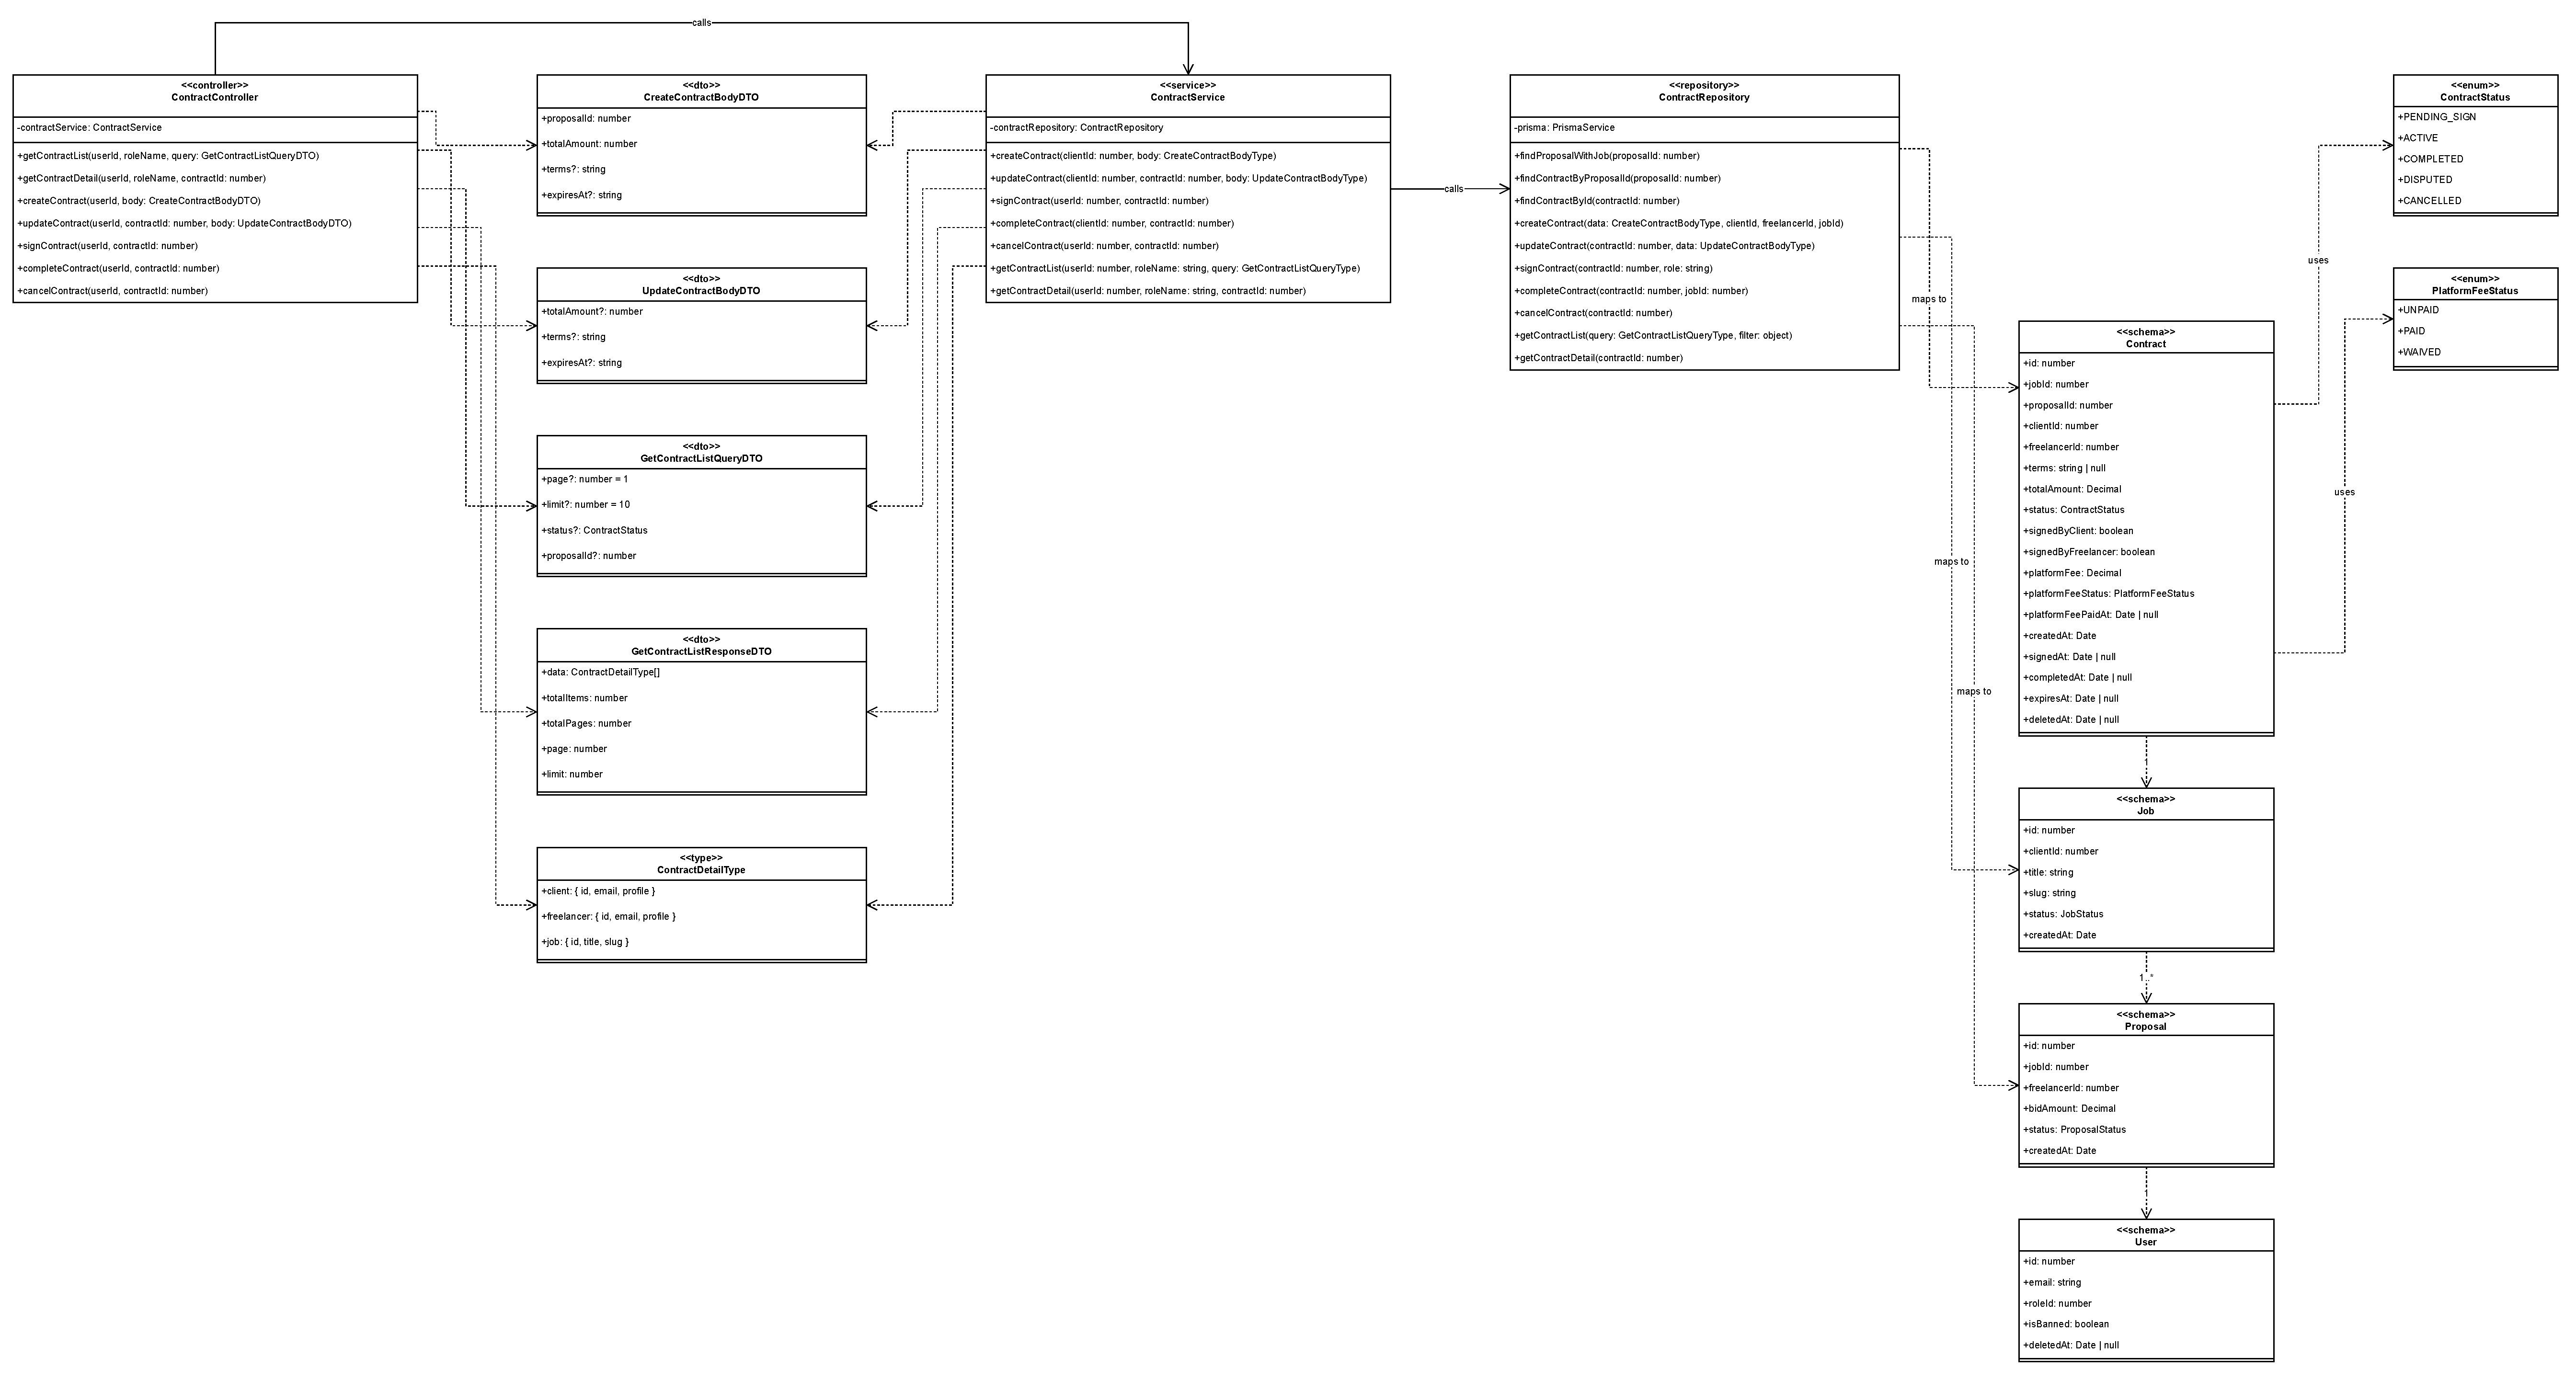
\includegraphics[width=0.92\textwidth, height=0.68\textheight, keepaspectratio]{../Report 4/images/sprint1/ntin/classDiagram/ContractManagement.pdf}
  \end{center}
\end{frame}

\begin{frame}[t]{Core Sequence -- Sign Contract}
  \framesubtitle{UC-13.06: Dual-Signature Verification, Ownership Guard \& Atomic State Transition}
  \begin{center}
    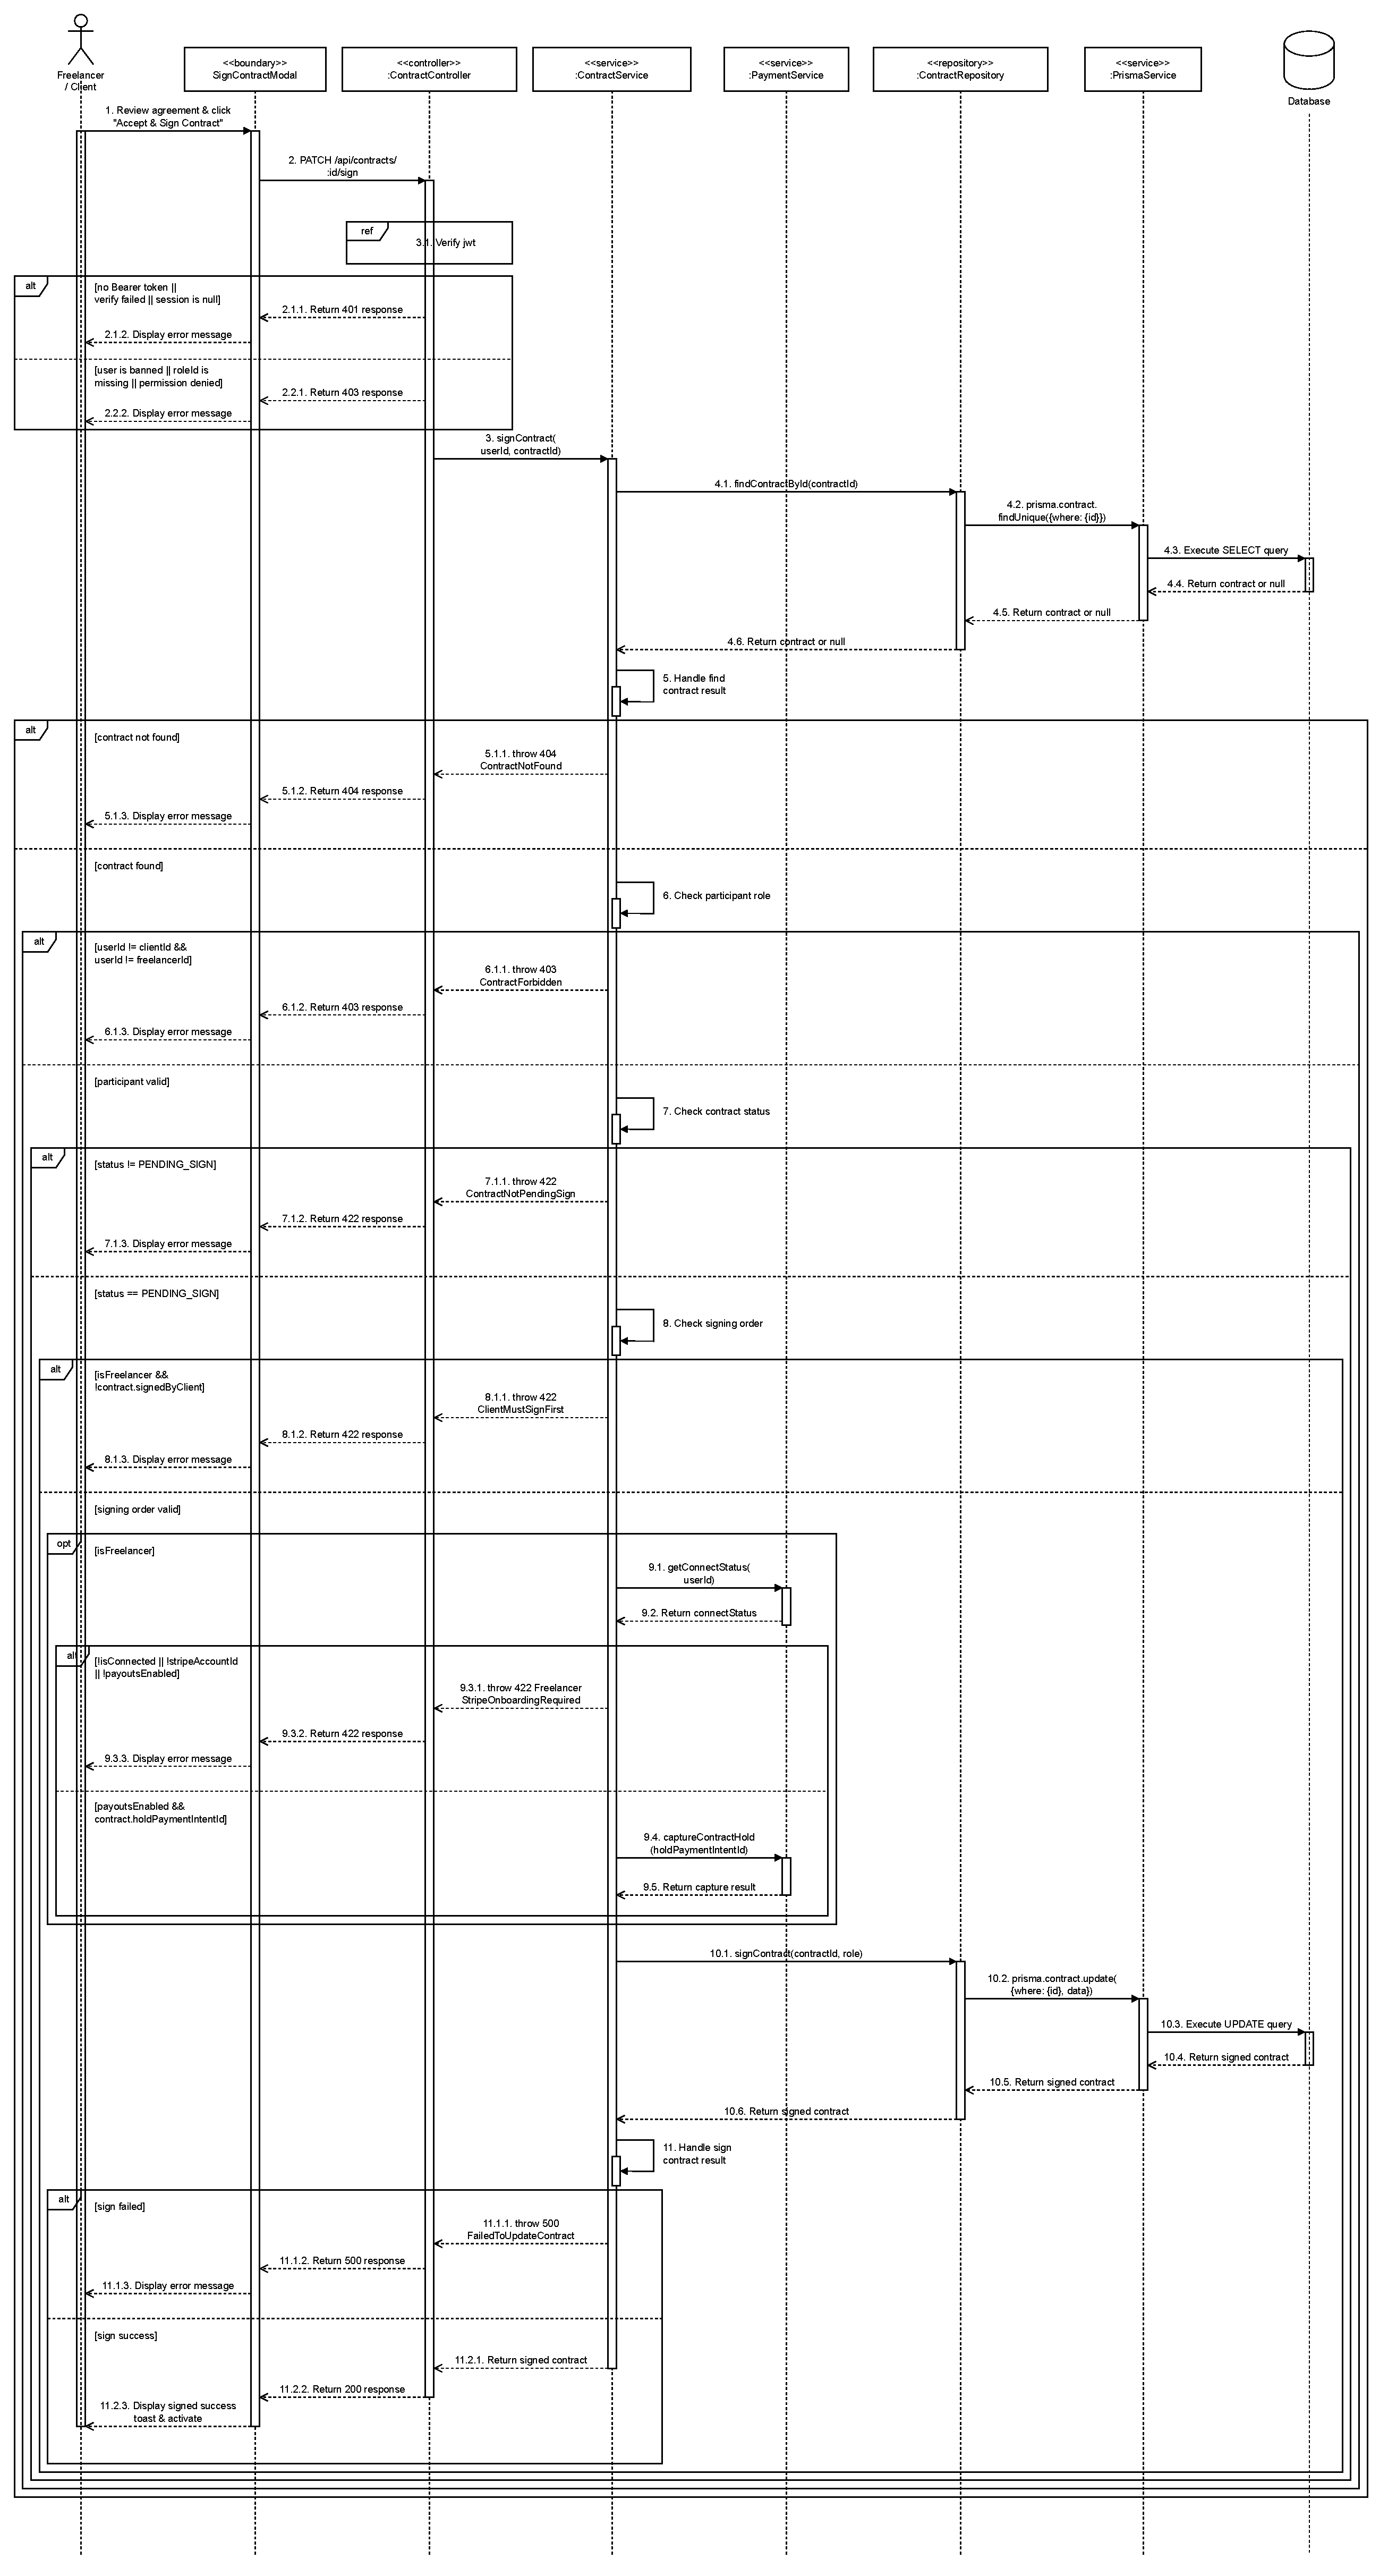
\includegraphics[width=0.92\textwidth, height=0.66\textheight, keepaspectratio]{../Report 4/images/sprint1/ntin/sequences/UC-13.06-sign-contract.pdf}
  \end{center}
\end{frame}

\begin{frame}[t]{Core Design -- Payment \& Escrow}
  \framesubtitle{Class Diagram: Stripe Connect, Escrow Hold, Release \& Webhook Handling (Report 4)}
  \begin{center}
    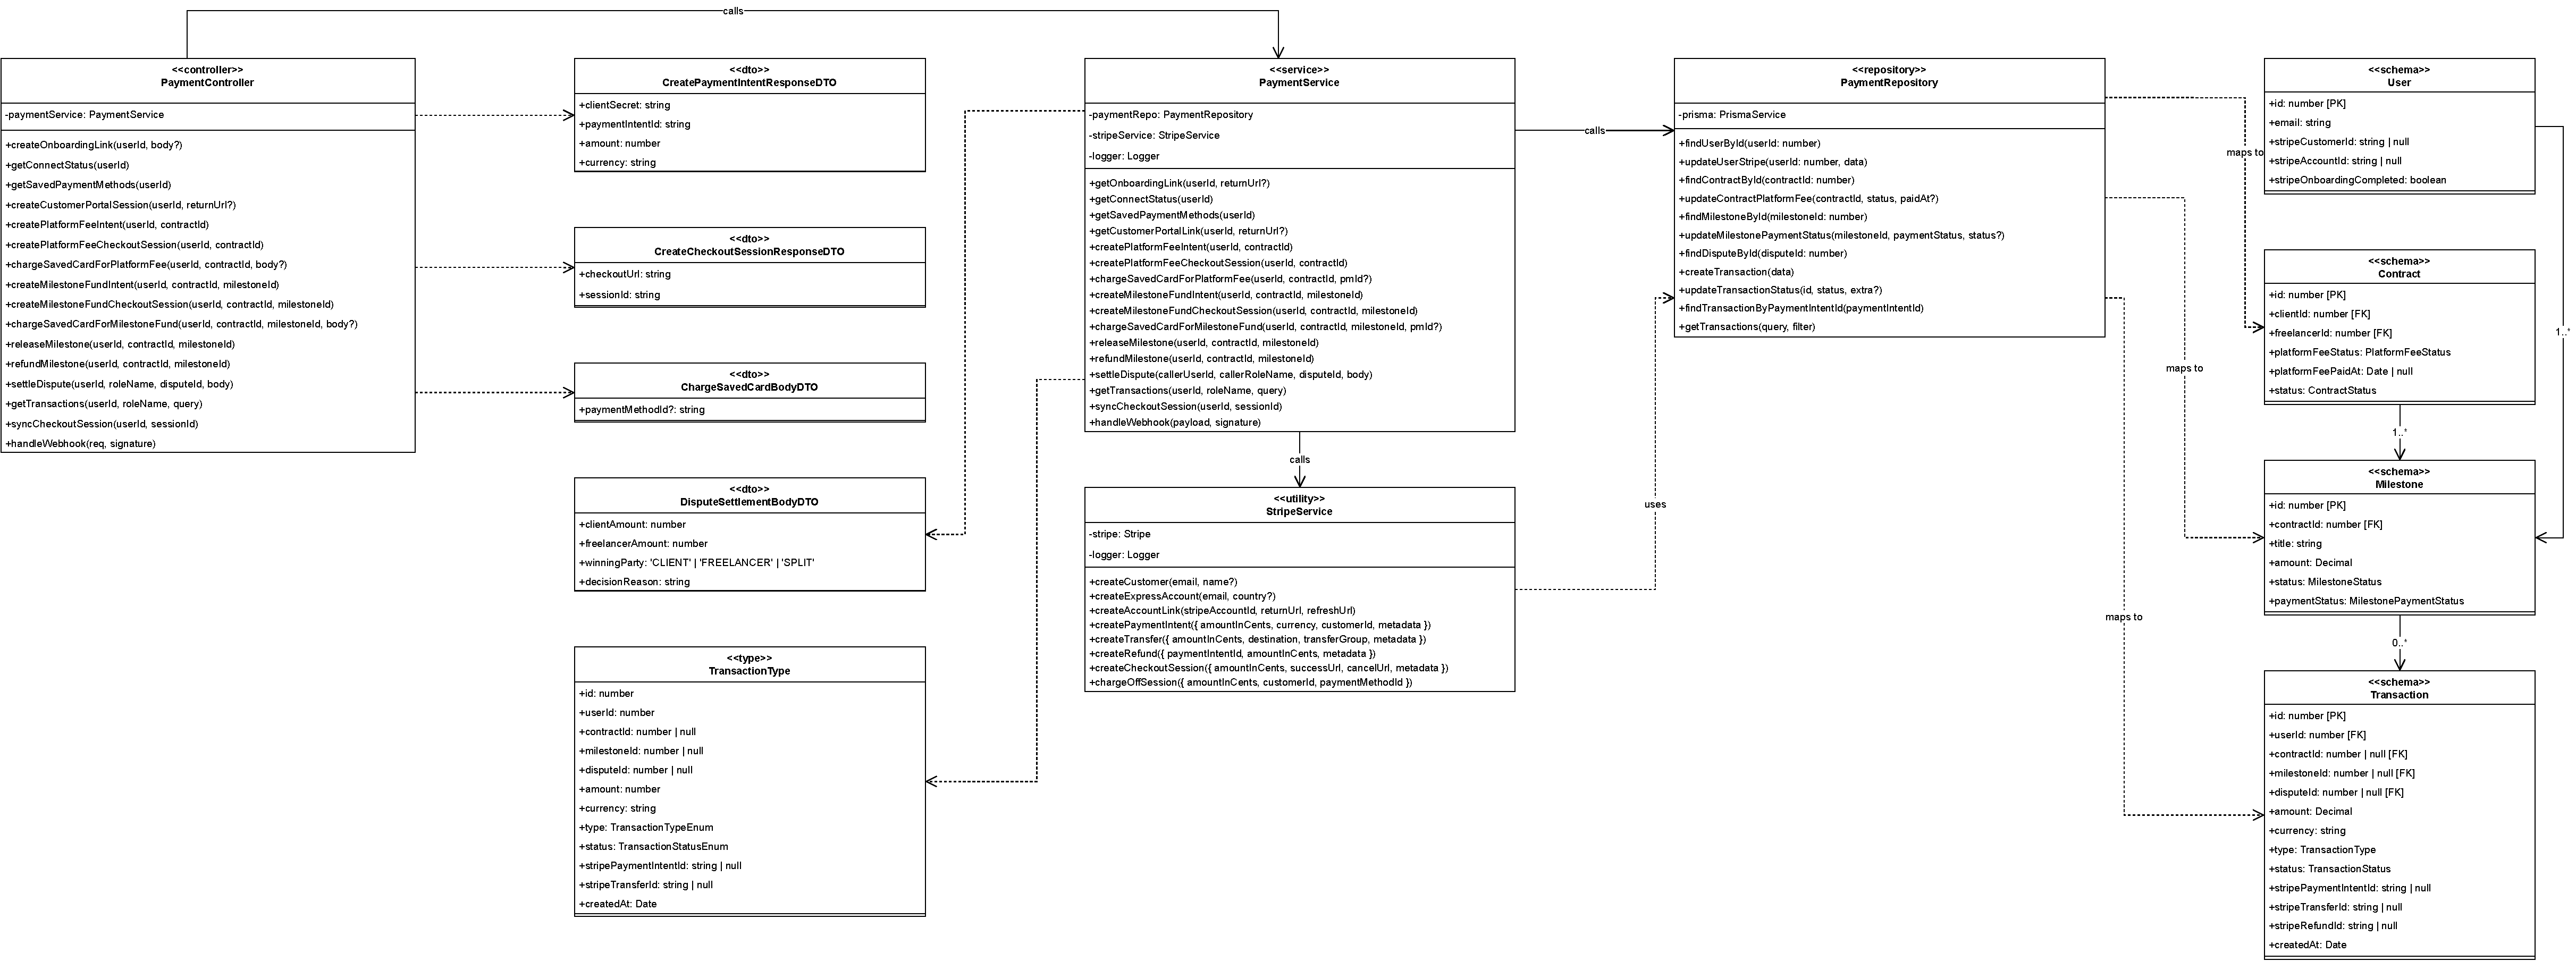
\includegraphics[width=0.92\textwidth, height=0.66\textheight, keepaspectratio]{../Report 4/images/sprint4/ntin/classDiagram/PaymentManagement.pdf}
  \end{center}
\end{frame}

\begin{frame}[t]{Core Sequence -- Release Escrow}
  \framesubtitle{UC-43.09: Milestone Approval, Stripe Transfer Payout \& Transaction Ledger Update}
  \begin{center}
    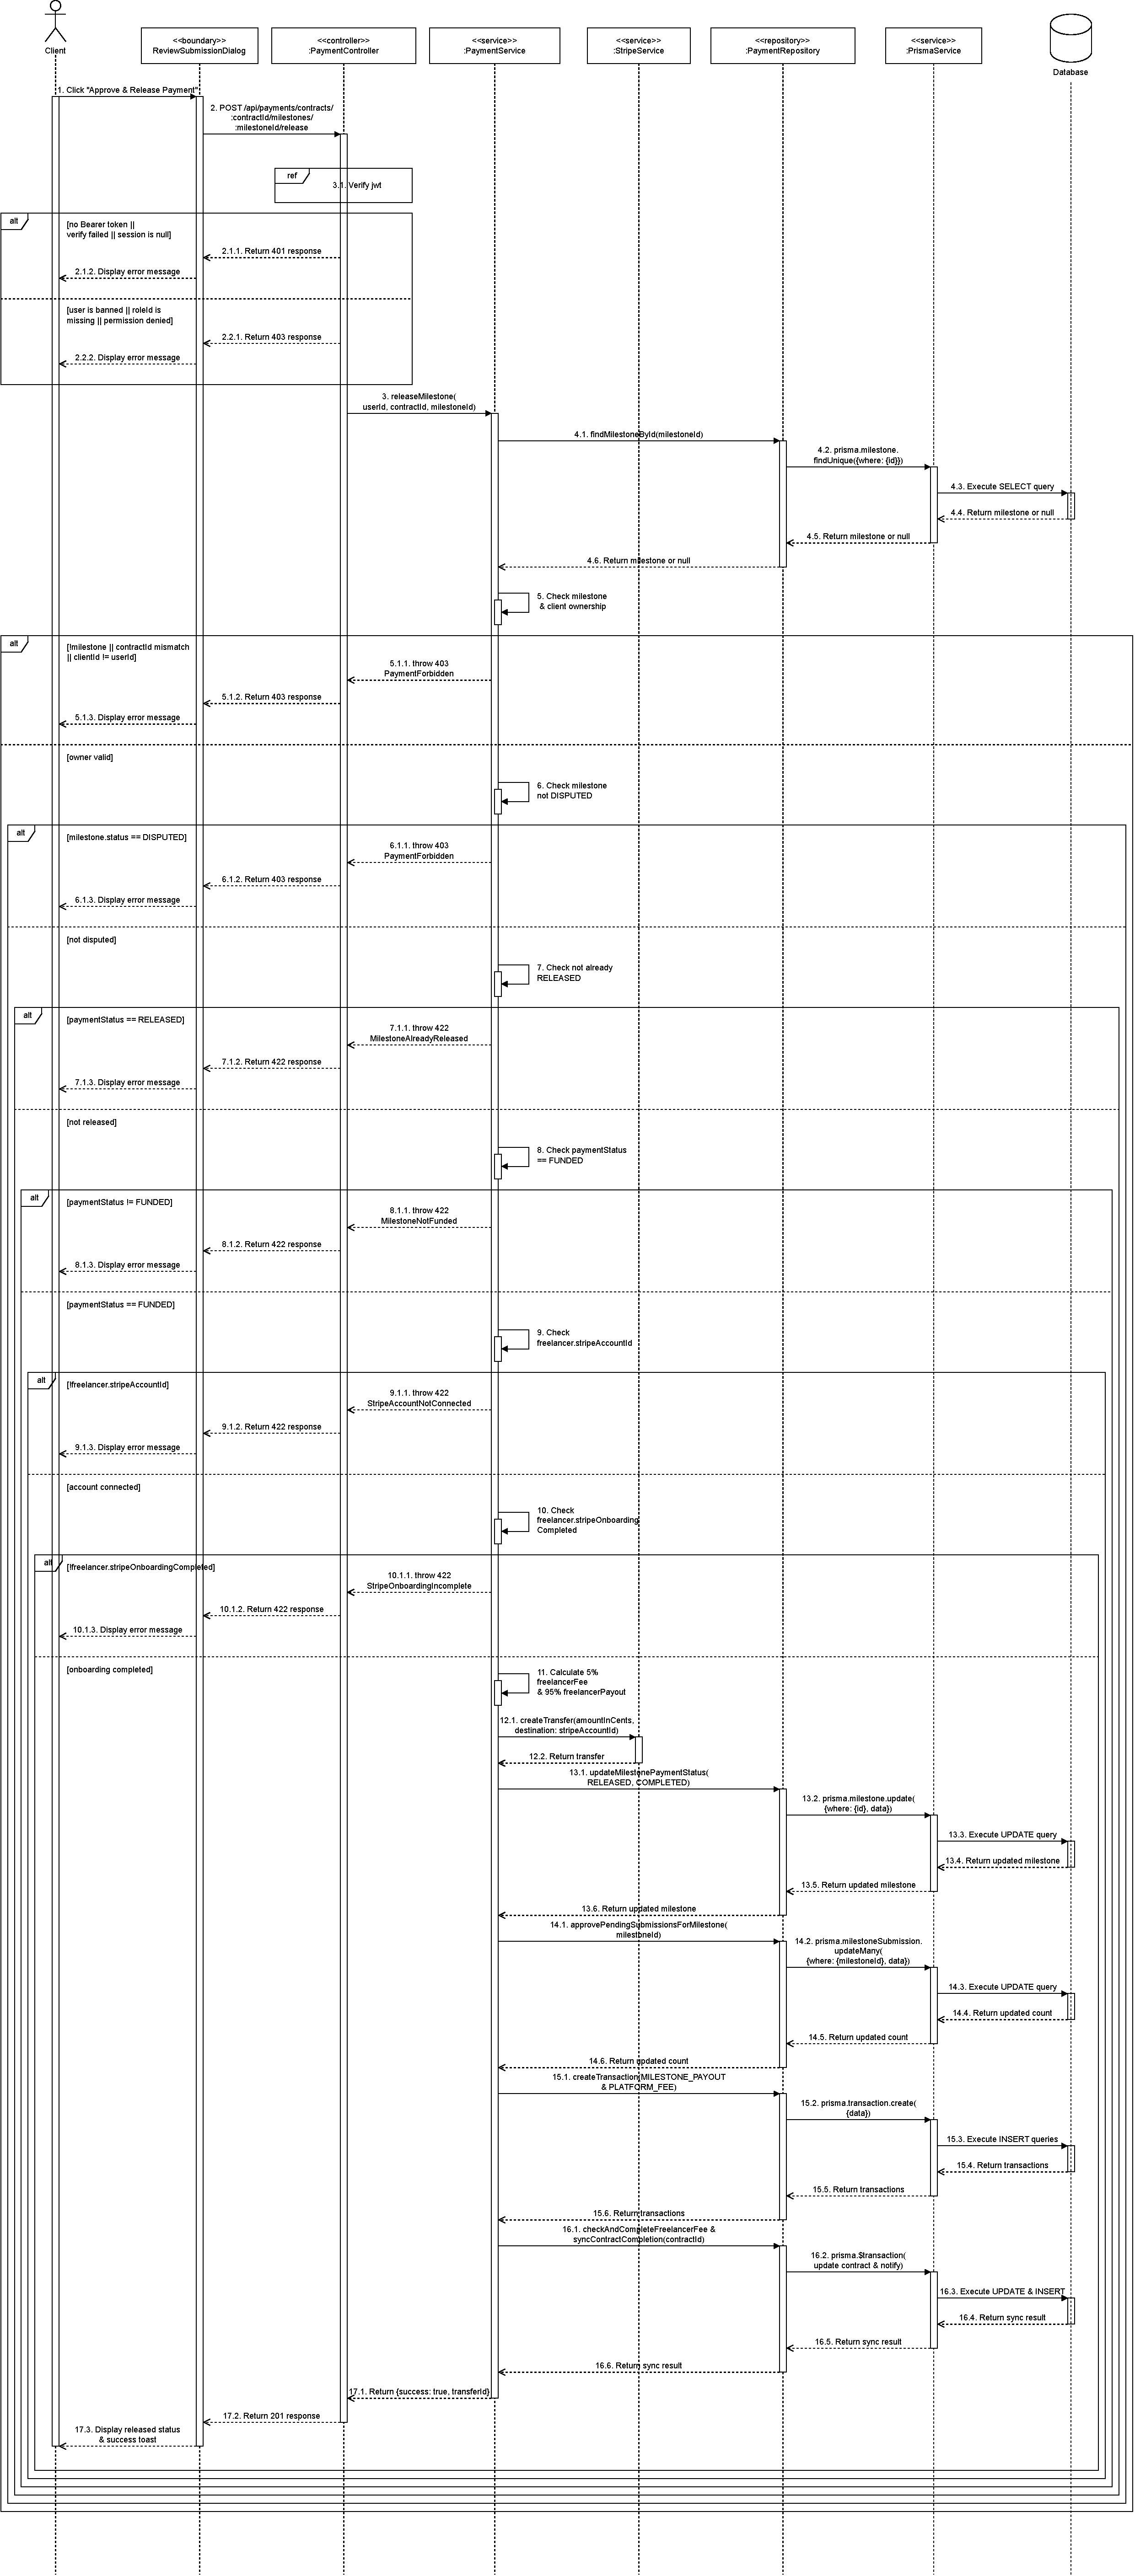
\includegraphics[width=0.92\textwidth, height=0.66\textheight, keepaspectratio]{../Report 4/images/sprint4/ntin/sequences/UC-43.09-release-milestone-escrow-payment.pdf}
  \end{center}
\end{frame}

% ==============================================================================
% CHAPTER V: SOFTWARE TESTING
% ==============================================================================
\chapterframe{CHAPTER V}{Software Testing}{Unit, Integration, System, and UAT Verification (Report 5 \& Report 7)}

\begin{frame}[t]{Test Execution Summary}
  \framesubtitle{2,984 Passed across 3,066 Test Cases (97.33\% Overall Execution) -- 0 Open Defects}
  \vspace{2pt}
  \renewcommand{\arraystretch}{1.2}
  \fontsize{9.2}{11.5}\selectfont
  \begin{tabularx}{\textwidth}{@{}X r r r r r@{}}
    \toprule
    \textcolor{fptaccent}{\textbf{Test Level}} & \textcolor{fptaccent}{\textbf{Total TCs}} & \textcolor{successgreen}{\textbf{Passed}} & \textcolor{fptaccent}{\textbf{Failed}} & \textcolor{fptgold}{\textbf{Pending}} & \textcolor{fptteal}{\textbf{Coverage}} \\
    \midrule
    Unit Testing (\texttt{UF-01}--\texttt{UF-246}) & 2,005 & 1,972 & 0 & 33 & 98.35\% \\
    Integration Testing & 84 & 84 & 0 & 0 & 100.00\% \\
    System Testing (44 Modules) & 935 & 886 & 0 & 49 & 94.76\% \\
    Acceptance Testing (UAT) & 42 & 42 & 0 & 0 & 100.00\% \\
    \midrule
    \textbf{Total} & \textbf{3,066} & \textbf{2,984} & \textbf{0} & \textbf{82} & \textbf{97.33\%} \\
    \bottomrule
  \end{tabularx}
  \vspace{4pt}
  \begin{columns}[T]
    \begin{column}{0.48\textwidth}
      \cardbox{6.5cm}{Automated Jest Backend Run}{%
        \texttt{Report5\_Unit\_Test\_Backend.html}: \textbf{1,536 / 1,536 passed} across \textbf{39 Jest suites} (Jest 30.0.0, \texttt{@nestjs/testing} 11.0.1).}
    \end{column}
    \begin{column}{0.48\textwidth}
      \cardbox{6.5cm}{Defect Resolution Rate (100\%)}{%
        \textbf{2 Critical}, \textbf{6 Major}, and \textbf{9 Minor} defects resolved prior to Sprint 5 (\textbf{0 open defects}).}
    \end{column}
  \end{columns}
\end{frame}

% ==============================================================================
% CHAPTER VI: RELEASE PACKAGE & USER GUIDE
% ==============================================================================
\chapterframe{CHAPTER VI}{Release Package \& User Guide}{5-Container Docker Compose Topology \& Bilingual Documentation}

\begin{frame}[t]{Production Deployment Topology \& Deliverables}
  \framesubtitle{Single-command boot via \texttt{docker compose up -d} with Infisical secrets}
  \begin{columns}[T]
    \begin{column}{0.55\textwidth}
      \renewcommand{\arraystretch}{1.3}
      \fontsize{8.0}{10.5}\selectfont
      \begin{tabular}{@{}l l l@{}}
        \toprule
        \textcolor{fptaccent}{\textbf{Container}} & \textcolor{fptaccent}{\textbf{Port}} & \textcolor{fptaccent}{\textbf{Role}} \\
        \midrule
        \texttt{frevia-frontend} & \texttt{3003:3000} & Next.js 16 Web \\
        \texttt{frevia-backend} & \texttt{3002:3000} & NestJS 11 API \\
        \texttt{frevia-cv-matching} & \texttt{8000:8000} & BGE-M3 + Chroma \\
        \texttt{frevia-id-verification} & \texttt{8001:8001} & eKYC OCR + Face \\
        \texttt{frevia-ollama} & \texttt{11434:11434} & Local \texttt{qwen3:4b} \\
        \bottomrule
      \end{tabular}\\[8pt]
      \textcolor{mutedgray}{\footnotesize External: PostgreSQL 16, Stripe Connect, Cloudinary, Google OAuth, SMTP}
    \end{column}
    \begin{column}{0.43\textwidth}
      \cardbox{5.8cm}{Release Artifacts (Report 6 \& 7)}{%
        \bul{Complete TypeScript monorepo (\texttt{apps/web}, \texttt{apps/api}, \texttt{packages/*}).}\\[4pt]
        \bul{Automated Prisma migrations \& deterministic seed scripts.}\\[4pt]
        \bul{Bilingual User Guides (EN/VI) with annotated UI walkthroughs across all 5 user roles.}
      }
    \end{column}
  \end{columns}
\end{frame}

% ==============================================================================
% CHAPTER VII: FUTURE WORK & CLOSING
% ==============================================================================
\chapterframe{CHAPTER VII}{Future Work \& Closing}{Strategic Roadmap and Live Demonstration}

\begin{frame}[t]{Strategic Future Directions}
  \framesubtitle{Planned enhancements beyond the initial release}
  \begin{columns}[T]
    \begin{column}{0.32\textwidth}
      \cardbox{4.2cm}{1. Multi-Rail Payments}{%
        Expand beyond Stripe USD to domestic Vietnamese gateways (VNPay, MoMo) and multi-currency settlement.}
    \end{column}
    \begin{column}{0.32\textwidth}
      \cardbox{4.2cm}{2. Edge AI Optimization}{%
        Apply INT8/INT4 quantization to local LLM and computer vision models to cut GPU/VRAM compute overhead.}
    \end{column}
    \begin{column}{0.32\textwidth}
      \cardbox{4.2cm}{3. Native Mobile \& Scale}{%
        Dedicated iOS/Android clients for native camera eKYC capture and Redis WebSocket adapters for multi-node scaling.}
    \end{column}
  \end{columns}
\end{frame}

% ==============================================================================
% THANK YOU SLIDE
% ==============================================================================
\begin{frame}[plain]
  \begin{tikzpicture}[remember picture, overlay]
    \fill[fptnavy] (current page.south west) rectangle (current page.north east);
    \draw[fptaccent, line width=2pt] ([xshift=-3cm,yshift=1.4cm]current page.center) -- ([xshift=3cm,yshift=1.4cm]current page.center);
    \node[anchor=center, font=\fontsize{38}{42}\selectfont\bfseries, text=white]
      at ([yshift=0.3cm]current page.center) {THANK YOU!};
    \node[anchor=center, font=\fontsize{14}{18}\selectfont, text=fptteal]
      at ([yshift=-0.75cm]current page.center) {Questions \& Live System Demonstration};
    \node[anchor=center, font=\fontsize{10.5}{14}\selectfont, text=lightgray]
      at ([yshift=-1.65cm]current page.center) {SEP490\_04 $\cdot$ FA26 $\cdot$ FREVIA};
  \end{tikzpicture}
\end{frame}

\end{document}
